\documentclass[1p]{elsarticle_modified}
%\bibliographystyle{elsarticle-num}

%\usepackage[colorlinks]{hyperref}
%\usepackage{abbrmath_seonhwa} %\Abb, \Ascr, \Acal ,\Abf, \Afrak
\usepackage{amsfonts}
\usepackage{amssymb}
\usepackage{amsmath}
\usepackage{amsthm}
\usepackage{scalefnt}
\usepackage{amsbsy}
\usepackage{kotex}
\usepackage{caption}
\usepackage{subfig}
\usepackage{color}
\usepackage{graphicx}
\usepackage{xcolor} %% white, black, red, green, blue, cyan, magenta, yellow
\usepackage{float}
\usepackage{setspace}
\usepackage{hyperref}

\usepackage{tikz}
\usetikzlibrary{arrows}

\usepackage{multirow}
\usepackage{array} % fixed length table
\usepackage{hhline}

%%%%%%%%%%%%%%%%%%%%%
\makeatletter
\renewcommand*\env@matrix[1][\arraystretch]{%
	\edef\arraystretch{#1}%
	\hskip -\arraycolsep
	\let\@ifnextchar\new@ifnextchar
	\array{*\c@MaxMatrixCols c}}
\makeatother %https://tex.stackexchange.com/questions/14071/how-can-i-increase-the-line-spacing-in-a-matrix
%%%%%%%%%%%%%%%

\usepackage[normalem]{ulem}

\newcommand{\msout}[1]{\ifmmode\text{\sout{\ensuremath{#1}}}\else\sout{#1}\fi}
%SOURCE: \msout is \stkout macro in https://tex.stackexchange.com/questions/20609/strikeout-in-math-mode

\newcommand{\cancel}[1]{
	\ifmmode
	{\color{red}\msout{#1}}
	\else
	{\color{red}\sout{#1}}
	\fi
}

\newcommand{\add}[1]{
	{\color{blue}\uwave{#1}}
}

\newcommand{\replace}[2]{
	\ifmmode
	{\color{red}\msout{#1}}{\color{blue}\uwave{#2}}
	\else
	{\color{red}\sout{#1}}{\color{blue}\uwave{#2}}
	\fi
}

\newcommand{\Sol}{\mathcal{S}} %segment
\newcommand{\D}{D} %diagram
\newcommand{\A}{\mathcal{A}} %arc


%%%%%%%%%%%%%%%%%%%%%%%%%%%%%5 test

\def\sl{\operatorname{\textup{SL}}(2,\Cbb)}
\def\psl{\operatorname{\textup{PSL}}(2,\Cbb)}
\def\quan{\mkern 1mu \triangleright \mkern 1mu}

\theoremstyle{definition}
\newtheorem{thm}{Theorem}[section]
\newtheorem{prop}[thm]{Proposition}
\newtheorem{lem}[thm]{Lemma}
\newtheorem{ques}[thm]{Question}
\newtheorem{cor}[thm]{Corollary}
\newtheorem{defn}[thm]{Definition}
\newtheorem{exam}[thm]{Example}
\newtheorem{rmk}[thm]{Remark}
\newtheorem{alg}[thm]{Algorithm}

\newcommand{\I}{\sqrt{-1}}
\begin{document}

%\begin{frontmatter}
%
%\title{Boundary parabolic representations of knots up to 8 crossings}
%
%%% Group authors per affiliation:
%\author{Yunhi Cho} 
%\address{Department of Mathematics, University of Seoul, Seoul, Korea}
%\ead{yhcho@uos.ac.kr}
%
%
%\author{Seonhwa Kim} %\fnref{s_kim}}
%\address{Center for Geometry and Physics, Institute for Basic Science, Pohang, 37673, Korea}
%\ead{ryeona17@ibs.re.kr}
%
%\author{Hyuk Kim}
%\address{Department of Mathematical Sciences, Seoul National University, Seoul 08826, Korea}
%\ead{hyukkim@snu.ac.kr}
%
%\author{Seokbeom Yoon}
%\address{Department of Mathematical Sciences, Seoul National University, Seoul, 08826,  Korea}
%\ead{sbyoon15@snu.ac.kr}
%
%\begin{abstract}
%We find all boundary parabolic representation of knots up to 8 crossings.
%
%\end{abstract}
%\begin{keyword}
%    \MSC[2010] 57M25 
%\end{keyword}
%
%\end{frontmatter}

%\linenumbers
%\tableofcontents
%
\newcommand\colored[1]{\textcolor{white}{\rule[-0.35ex]{0.8em}{1.4ex}}\kern-0.8em\color{red} #1}%
%\newcommand\colored[1]{\textcolor{white}{ #1}\kern-2.17ex	\textcolor{white}{ #1}\kern-1.81ex	\textcolor{white}{ #1}\kern-2.15ex\color{red}#1	}

{\Large $\underline{12a_{0408}~(K12a_{0408})}$}

\setlength{\tabcolsep}{10pt}
\renewcommand{\arraystretch}{1.6}
\vspace{1cm}\begin{tabular}{m{100pt}>{\centering\arraybackslash}m{274pt}}
\multirow{5}{120pt}{
	\centering
	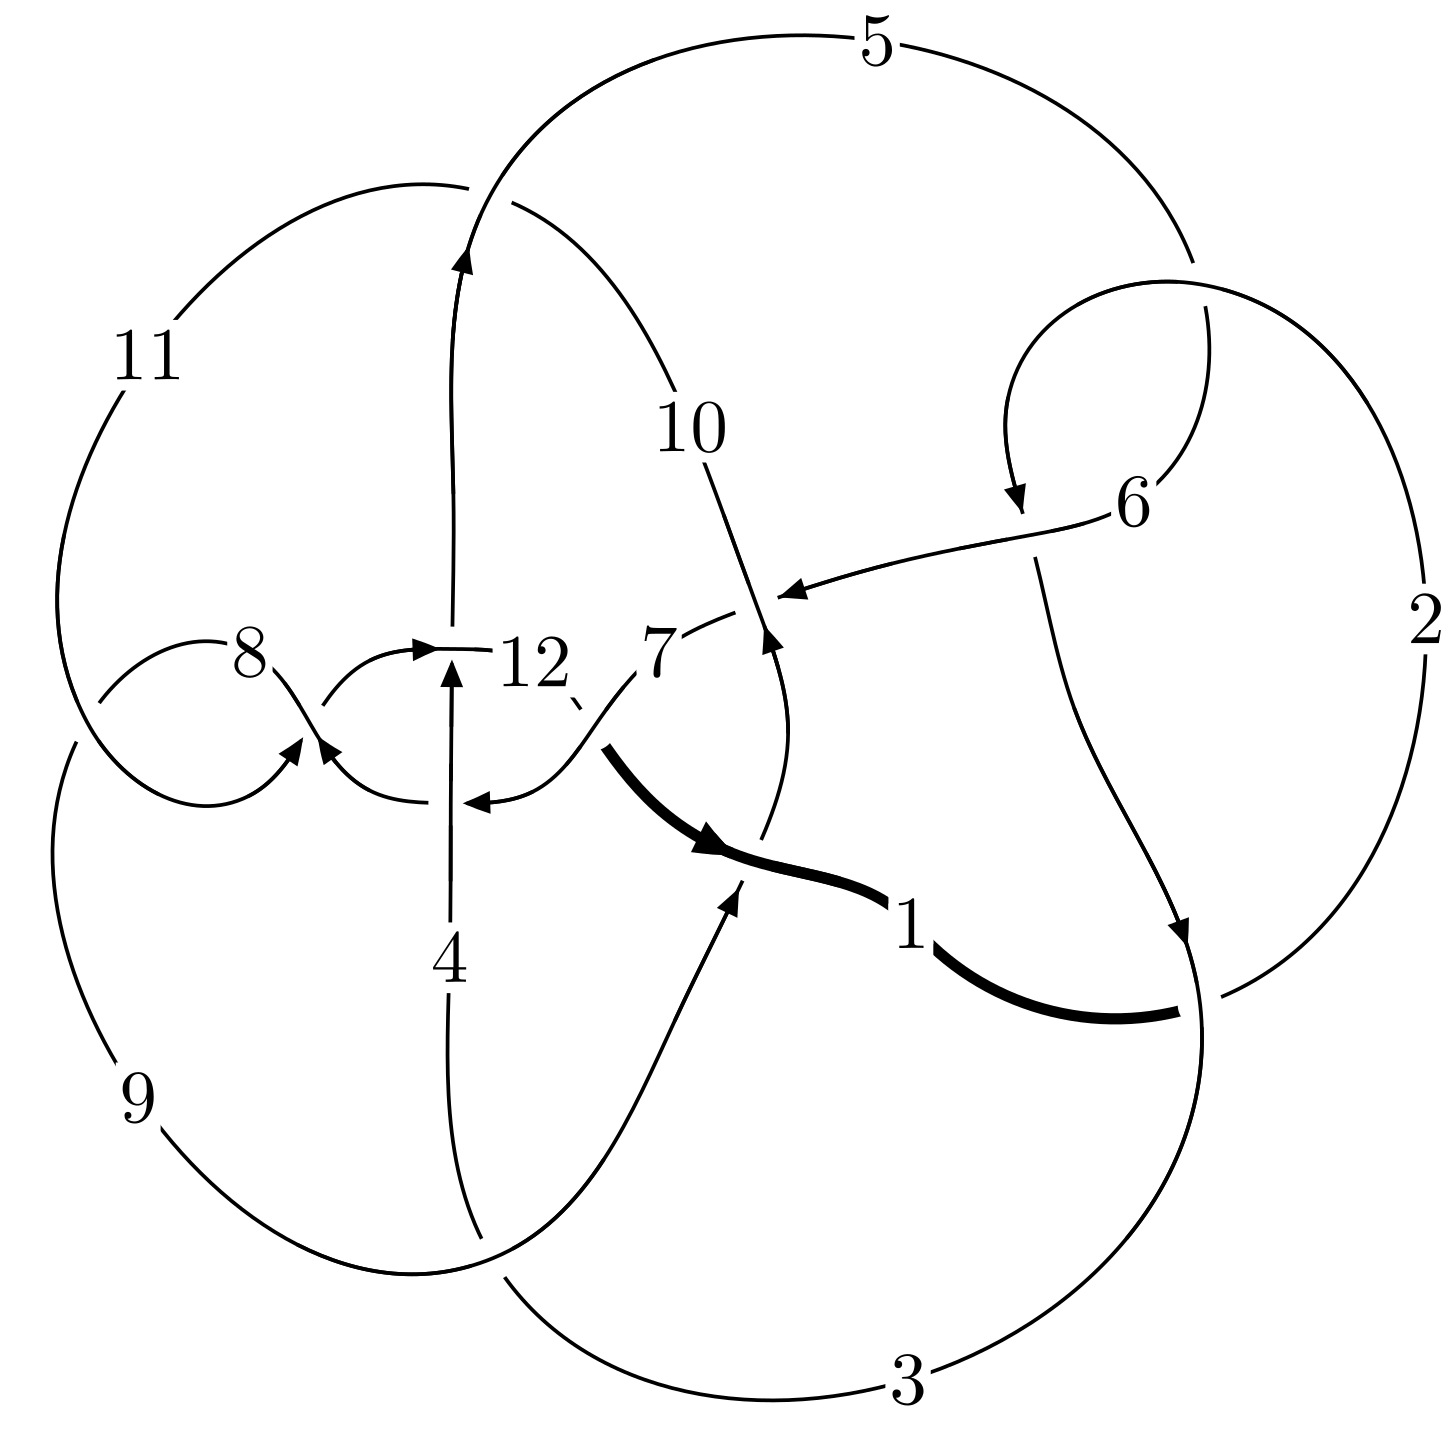
\includegraphics[width=112pt]{../../../GIT/diagram.site/Diagrams/png/1209_12a_0408.png}\\
\ \ \ A knot diagram\footnotemark}&
\allowdisplaybreaks
\textbf{Linearized knot diagam} \\
\cline{2-2}
 &
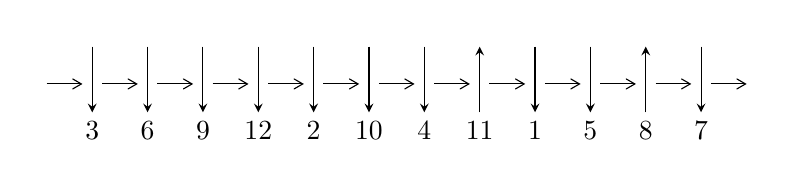
\begin{tikzpicture}[x=20pt, y=17pt]
	% nodes
	\node (C0) at (0, 0) {};
	\node (C1) at (1, 0) {};
	\node (C1U) at (1, +1) {};
	\node (C1D) at (1, -1) {3};

	\node (C2) at (2, 0) {};
	\node (C2U) at (2, +1) {};
	\node (C2D) at (2, -1) {6};

	\node (C3) at (3, 0) {};
	\node (C3U) at (3, +1) {};
	\node (C3D) at (3, -1) {9};

	\node (C4) at (4, 0) {};
	\node (C4U) at (4, +1) {};
	\node (C4D) at (4, -1) {12};

	\node (C5) at (5, 0) {};
	\node (C5U) at (5, +1) {};
	\node (C5D) at (5, -1) {2};

	\node (C6) at (6, 0) {};
	\node (C6U) at (6, +1) {};
	\node (C6D) at (6, -1) {10};

	\node (C7) at (7, 0) {};
	\node (C7U) at (7, +1) {};
	\node (C7D) at (7, -1) {4};

	\node (C8) at (8, 0) {};
	\node (C8U) at (8, +1) {};
	\node (C8D) at (8, -1) {11};

	\node (C9) at (9, 0) {};
	\node (C9U) at (9, +1) {};
	\node (C9D) at (9, -1) {1};

	\node (C10) at (10, 0) {};
	\node (C10U) at (10, +1) {};
	\node (C10D) at (10, -1) {5};

	\node (C11) at (11, 0) {};
	\node (C11U) at (11, +1) {};
	\node (C11D) at (11, -1) {8};

	\node (C12) at (12, 0) {};
	\node (C12U) at (12, +1) {};
	\node (C12D) at (12, -1) {7};
	\node (C13) at (13, 0) {};

	% arrows
	\draw[->,>={angle 60}]
	(C0) edge (C1) (C1) edge (C2) (C2) edge (C3) (C3) edge (C4) (C4) edge (C5) (C5) edge (C6) (C6) edge (C7) (C7) edge (C8) (C8) edge (C9) (C9) edge (C10) (C10) edge (C11) (C11) edge (C12) (C12) edge (C13) ;	\draw[->,>=stealth]
	(C1U) edge (C1D) (C2U) edge (C2D) (C3U) edge (C3D) (C4U) edge (C4D) (C5U) edge (C5D) (C6U) edge (C6D) (C7U) edge (C7D) (C8D) edge (C8U) (C9U) edge (C9D) (C10U) edge (C10D) (C11D) edge (C11U) (C12U) edge (C12D) ;
	\end{tikzpicture} \\
\hhline{~~} \\& 
\textbf{Solving Sequence} \\ \cline{2-2} 
 &
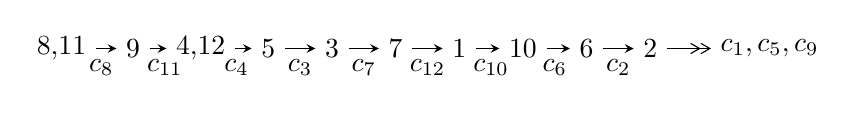
\begin{tikzpicture}[x=23pt, y=7pt]
	% node
	\node (A0) at (-1/8, 0) {8,11};
	\node (A1) at (1, 0) {9};
	\node (A2) at (33/16, 0) {4,12};
	\node (A3) at (25/8, 0) {5};
	\node (A4) at (33/8, 0) {3};
	\node (A5) at (41/8, 0) {7};
	\node (A6) at (49/8, 0) {1};
	\node (A7) at (57/8, 0) {10};
	\node (A8) at (65/8, 0) {6};
	\node (A9) at (73/8, 0) {2};
	\node (C1) at (1/2, -1) {$c_{8}$};
	\node (C2) at (3/2, -1) {$c_{11}$};
	\node (C3) at (21/8, -1) {$c_{4}$};
	\node (C4) at (29/8, -1) {$c_{3}$};
	\node (C5) at (37/8, -1) {$c_{7}$};
	\node (C6) at (45/8, -1) {$c_{12}$};
	\node (C7) at (53/8, -1) {$c_{10}$};
	\node (C8) at (61/8, -1) {$c_{6}$};
	\node (C9) at (69/8, -1) {$c_{2}$};
	\node (A10) at (11, 0) {$c_{1},c_{5},c_{9}$};

	% edge
	\draw[->,>=stealth]	
	(A0) edge (A1) (A1) edge (A2) (A2) edge (A3) (A3) edge (A4) (A4) edge (A5) (A5) edge (A6) (A6) edge (A7) (A7) edge (A8) (A8) edge (A9) ;
	\draw[->>,>={angle 60}]	
	(A9) edge (A10);
\end{tikzpicture} \\ 

\end{tabular} \\

\footnotetext{
The image of knot diagram is generated by the software ``\textbf{Draw programme}" developed by Andrew Bartholomew(\url{http://www.layer8.co.uk/maths/draw/index.htm\#Running-draw}), where we modified some parts for our purpose(\url{https://github.com/CATsTAILs/LinksPainter}).
}\phantom \\ \newline 
\centering \textbf{Ideals for irreducible components\footnotemark of $X_{\text{par}}$} 
 
\begin{align*}
I^u_{1}&=\langle 
-5.94883\times10^{82} u^{65}+1.44814\times10^{84} u^{64}+\cdots+5.09401\times10^{83} b-2.12573\times10^{85},\\
\phantom{I^u_{1}}&\phantom{= \langle  }-4.92961\times10^{84} u^{65}+1.25631\times10^{86} u^{64}+\cdots+3.31110\times10^{85} a+5.80286\times10^{87},\\
\phantom{I^u_{1}}&\phantom{= \langle  }u^{66}-26 u^{65}+\cdots-29690 u+1300\rangle \\
I^u_{2}&=\langle 
817219108 u^{29} a^3+512017417 u^{29} a^2+\cdots+807804715 a+597442347,\\
\phantom{I^u_{2}}&\phantom{= \langle  }16 u^{29} a^2-224 u^{29} a+\cdots-1933 a+10413,\;u^{30}+9 u^{29}+\cdots+14 u+1\rangle \\
I^u_{3}&=\langle 
2.05685\times10^{15} u^{35}+3.17765\times10^{16} u^{34}+\cdots+1.33360\times10^{16} b+3.92713\times10^{16},\\
\phantom{I^u_{3}}&\phantom{= \langle  }-2.48733\times10^{16} u^{35}-3.52235\times10^{17} u^{34}+\cdots+9.33523\times10^{16} a-1.32132\times10^{18},\\
\phantom{I^u_{3}}&\phantom{= \langle  }u^{36}+15 u^{35}+\cdots+100 u+7\rangle \\
I^u_{4}&=\langle 
-8 a^3 u-6 a^3-3 a^2 u-21 a^2+59 a u+50 b-37 a+13 u+41,\\
\phantom{I^u_{4}}&\phantom{= \langle  }a^4- a^3 u+a^3-3 a^2 u-4 a^2+3 a u- a+2 u+3,\;u^2+1\rangle \\
\\
\end{align*}
\raggedright * 4 irreducible components of $\dim_{\mathbb{C}}=0$, with total 230 representations.\\
\footnotetext{All coefficients of polynomials are rational numbers. But the coefficients are sometimes approximated in decimal forms when there is not enough margin.}
\newpage
\renewcommand{\arraystretch}{1}
\centering \section*{I. $I^u_{1}= \langle -5.95\times10^{82} u^{65}+1.45\times10^{84} u^{64}+\cdots+5.09\times10^{83} b-2.13\times10^{85},\;-4.93\times10^{84} u^{65}+1.26\times10^{86} u^{64}+\cdots+3.31\times10^{85} a+5.80\times10^{87},\;u^{66}-26 u^{65}+\cdots-29690 u+1300 \rangle$}
\flushleft \textbf{(i) Arc colorings}\\
\begin{tabular}{m{7pt} m{180pt} m{7pt} m{180pt} }
\flushright $a_{8}=$&$\begin{pmatrix}1\\0\end{pmatrix}$ \\
\flushright $a_{11}=$&$\begin{pmatrix}0\\u\end{pmatrix}$ \\
\flushright $a_{9}=$&$\begin{pmatrix}1\\- u^2\end{pmatrix}$ \\
\flushright $a_{4}=$&$\begin{pmatrix}0.148881 u^{65}-3.79422 u^{64}+\cdots+3912.79 u-175.254\\0.116781 u^{65}-2.84284 u^{64}+\cdots-736.065 u+41.7300\end{pmatrix}$ \\
\flushright $a_{12}=$&$\begin{pmatrix}u\\u\end{pmatrix}$ \\
\flushright $a_{5}=$&$\begin{pmatrix}-0.0445864 u^{65}+1.18662 u^{64}+\cdots+403.833 u-23.4390\\-0.0766864 u^{65}+2.13800 u^{64}+\cdots-4245.02 u+193.545\end{pmatrix}$ \\
\flushright $a_{3}=$&$\begin{pmatrix}0.121508 u^{65}-3.33673 u^{64}+\cdots+5260.00 u-233.217\\0.407157 u^{65}-10.5042 u^{64}+\cdots+6775.86 u-288.744\end{pmatrix}$ \\
\flushright $a_{7}=$&$\begin{pmatrix}-0.0389164 u^{65}+1.01371 u^{64}+\cdots-1316.21 u+61.4204\\-0.0414582 u^{65}+1.03834 u^{64}+\cdots-132.582 u+3.30431\end{pmatrix}$ \\
\flushright $a_{1}=$&$\begin{pmatrix}0.197987 u^{65}-4.99729 u^{64}+\cdots+2699.62 u-115.833\\0.159022 u^{65}-3.78559 u^{64}+\cdots-2163.10 u+104.551\end{pmatrix}$ \\
\flushright $a_{10}=$&$\begin{pmatrix}-0.00561786 u^{65}+0.162911 u^{64}+\cdots-830.706 u+38.6946\\-0.00627711 u^{65}+0.204138 u^{64}+\cdots-741.092 u+32.1698\end{pmatrix}$ \\
\flushright $a_{6}=$&$\begin{pmatrix}-0.0826048 u^{65}+2.15913 u^{64}+\cdots-2200.04 u+99.6941\\-0.141191 u^{65}+3.59078 u^{64}+\cdots-2245.40 u+96.5869\end{pmatrix}$ \\
\flushright $a_{2}=$&$\begin{pmatrix}-0.0628923 u^{65}+1.60318 u^{64}+\cdots-1571.82 u+67.8794\\0.00840374 u^{65}-0.102004 u^{64}+\cdots-1483.96 u+65.7618\end{pmatrix}$\\&\end{tabular}
\flushleft \textbf{(ii) Obstruction class $= -1$}\\~\\
\flushleft \textbf{(iii) Cusp Shapes $= -0.953489 u^{65}+23.7173 u^{64}+\cdots-15544.8 u+676.189$}\\~\\
\newpage\renewcommand{\arraystretch}{1}
\flushleft \textbf{(iv) u-Polynomials at the component}\newline \\
\begin{tabular}{m{50pt}|m{274pt}}
Crossings & \hspace{64pt}u-Polynomials at each crossing \\
\hline $$\begin{aligned}c_{1}\end{aligned}$$&$\begin{aligned}
&u^{66}+31 u^{65}+\cdots+17676 u+2704
\end{aligned}$\\
\hline $$\begin{aligned}c_{2},c_{5}\end{aligned}$$&$\begin{aligned}
&u^{66}+13 u^{65}+\cdots-738 u-52
\end{aligned}$\\
\hline $$\begin{aligned}c_{3},c_{10}\end{aligned}$$&$\begin{aligned}
&u^{66}+13 u^{64}+\cdots+37 u-181
\end{aligned}$\\
\hline $$\begin{aligned}c_{4},c_{7}\end{aligned}$$&$\begin{aligned}
&u^{66}-15 u^{64}+\cdots- u-1
\end{aligned}$\\
\hline $$\begin{aligned}c_{6},c_{9}\end{aligned}$$&$\begin{aligned}
&u^{66}+2 u^{65}+\cdots+5 u+2
\end{aligned}$\\
\hline $$\begin{aligned}c_{8},c_{11}\end{aligned}$$&$\begin{aligned}
&u^{66}+26 u^{65}+\cdots+29690 u+1300
\end{aligned}$\\
\hline $$\begin{aligned}c_{12}\end{aligned}$$&$\begin{aligned}
&u^{66}+56 u^{65}+\cdots+17045651456 u+536870912
\end{aligned}$\\
\hline
\end{tabular}\\~\\
\newpage\renewcommand{\arraystretch}{1}
\flushleft \textbf{(v) Riley Polynomials at the component}\newline \\
\begin{tabular}{m{50pt}|m{274pt}}
Crossings & \hspace{64pt}Riley Polynomials at each crossing \\
\hline $$\begin{aligned}c_{1}\end{aligned}$$&$\begin{aligned}
&y^{66}+17 y^{65}+\cdots-505176688 y+7311616
\end{aligned}$\\
\hline $$\begin{aligned}c_{2},c_{5}\end{aligned}$$&$\begin{aligned}
&y^{66}-31 y^{65}+\cdots-17676 y+2704
\end{aligned}$\\
\hline $$\begin{aligned}c_{3},c_{10}\end{aligned}$$&$\begin{aligned}
&y^{66}+26 y^{65}+\cdots+13111 y+32761
\end{aligned}$\\
\hline $$\begin{aligned}c_{4},c_{7}\end{aligned}$$&$\begin{aligned}
&y^{66}-30 y^{65}+\cdots-51 y+1
\end{aligned}$\\
\hline $$\begin{aligned}c_{6},c_{9}\end{aligned}$$&$\begin{aligned}
&y^{66}-2 y^{65}+\cdots+43 y+4
\end{aligned}$\\
\hline $$\begin{aligned}c_{8},c_{11}\end{aligned}$$&$\begin{aligned}
&y^{66}+46 y^{65}+\cdots+26109300 y+1690000
\end{aligned}$\\
\hline $$\begin{aligned}c_{12}\end{aligned}$$&$\begin{aligned}
&y^{66}+6 y^{65}+\cdots-1242993497154256896 y+288230376151711744
\end{aligned}$\\
\hline
\end{tabular}\\~\\
\newpage\flushleft \textbf{(vi) Complex Volumes and Cusp Shapes}
$$\begin{array}{c|c|c}  
\text{Solutions to }I^u_{1}& \I (\text{vol} + \sqrt{-1}CS) & \text{Cusp shape}\\
 \hline 
\begin{aligned}
u &= \phantom{-}0.965644 + 0.116585 I \\
a &= -0.128217 + 0.077481 I \\
b &= \phantom{-}0.781461 + 0.909186 I\end{aligned}
 & \phantom{-}0.04153 - 7.33110 I & \phantom{-0.000000 } 0 \\ \hline\begin{aligned}
u &= \phantom{-}0.965644 - 0.116585 I \\
a &= -0.128217 - 0.077481 I \\
b &= \phantom{-}0.781461 - 0.909186 I\end{aligned}
 & \phantom{-}0.04153 + 7.33110 I & \phantom{-0.000000 } 0 \\ \hline\begin{aligned}
u &= \phantom{-}0.968871\phantom{ +0.000000I} \\
a &= \phantom{-}0.0216859\phantom{ +0.000000I} \\
b &= -0.674970\phantom{ +0.000000I}\end{aligned}
 & -4.57047\phantom{ +0.000000I} & \phantom{-0.000000 } 0 \\ \hline\begin{aligned}
u &= -0.107773 + 0.943078 I \\
a &= -2.13279 - 0.30507 I \\
b &= -1.152450 + 0.804909 I\end{aligned}
 & -1.36529 - 0.47729 I & \phantom{-0.000000 } 0 \\ \hline\begin{aligned}
u &= -0.107773 - 0.943078 I \\
a &= -2.13279 + 0.30507 I \\
b &= -1.152450 - 0.804909 I\end{aligned}
 & -1.36529 + 0.47729 I & \phantom{-0.000000 } 0 \\ \hline\begin{aligned}
u &= -0.191979 + 0.928389 I \\
a &= -1.20721 - 0.75473 I \\
b &= -0.883784 + 0.130347 I\end{aligned}
 & -1.54285 - 0.80188 I & \phantom{-0.000000 } 0 \\ \hline\begin{aligned}
u &= -0.191979 - 0.928389 I \\
a &= -1.20721 + 0.75473 I \\
b &= -0.883784 - 0.130347 I\end{aligned}
 & -1.54285 + 0.80188 I & \phantom{-0.000000 } 0 \\ \hline\begin{aligned}
u &= -0.212483 + 1.044600 I \\
a &= \phantom{-}1.297590 + 0.542475 I \\
b &= \phantom{-}0.904573 - 0.243533 I\end{aligned}
 & -2.15381 - 4.98396 I & \phantom{-0.000000 } 0 \\ \hline\begin{aligned}
u &= -0.212483 - 1.044600 I \\
a &= \phantom{-}1.297590 - 0.542475 I \\
b &= \phantom{-}0.904573 + 0.243533 I\end{aligned}
 & -2.15381 + 4.98396 I & \phantom{-0.000000 } 0 \\ \hline\begin{aligned}
u &= \phantom{-}0.064628 + 1.072060 I \\
a &= \phantom{-}1.87038 + 0.10819 I \\
b &= \phantom{-}1.06339 - 0.93238 I\end{aligned}
 & -2.26306 + 0.50106 I & \phantom{-0.000000 } 0\\
 \hline 
 \end{array}$$\newpage$$\begin{array}{c|c|c}  
\text{Solutions to }I^u_{1}& \I (\text{vol} + \sqrt{-1}CS) & \text{Cusp shape}\\
 \hline 
\begin{aligned}
u &= \phantom{-}0.064628 - 1.072060 I \\
a &= \phantom{-}1.87038 - 0.10819 I \\
b &= \phantom{-}1.06339 + 0.93238 I\end{aligned}
 & -2.26306 - 0.50106 I & \phantom{-0.000000 } 0 \\ \hline\begin{aligned}
u &= -0.038288 + 1.076850 I \\
a &= -2.00469 - 0.14451 I \\
b &= -1.14404 + 0.88729 I\end{aligned}
 & -2.15487 + 3.80132 I & \phantom{-0.000000 } 0 \\ \hline\begin{aligned}
u &= -0.038288 - 1.076850 I \\
a &= -2.00469 + 0.14451 I \\
b &= -1.14404 - 0.88729 I\end{aligned}
 & -2.15487 - 3.80132 I & \phantom{-0.000000 } 0 \\ \hline\begin{aligned}
u &= \phantom{-}1.000080 + 0.415641 I \\
a &= \phantom{-}0.190224 - 0.401848 I \\
b &= -0.776510 - 0.859685 I\end{aligned}
 & \phantom{-}5.94107 - 4.21086 I & \phantom{-0.000000 } 0 \\ \hline\begin{aligned}
u &= \phantom{-}1.000080 - 0.415641 I \\
a &= \phantom{-}0.190224 + 0.401848 I \\
b &= -0.776510 + 0.859685 I\end{aligned}
 & \phantom{-}5.94107 + 4.21086 I & \phantom{-0.000000 } 0 \\ \hline\begin{aligned}
u &= -0.068173 + 1.089420 I \\
a &= \phantom{-}1.312090 + 0.193562 I \\
b &= \phantom{-}0.800595 - 0.509315 I\end{aligned}
 & -3.63493 + 0.26678 I & \phantom{-0.000000 } 0 \\ \hline\begin{aligned}
u &= -0.068173 - 1.089420 I \\
a &= \phantom{-}1.312090 - 0.193562 I \\
b &= \phantom{-}0.800595 + 0.509315 I\end{aligned}
 & -3.63493 - 0.26678 I & \phantom{-0.000000 } 0 \\ \hline\begin{aligned}
u &= -1.059830 + 0.271315 I \\
a &= -0.146768 + 0.536946 I \\
b &= -0.042981 + 0.289942 I\end{aligned}
 & \phantom{-}2.65184 - 2.70646 I & \phantom{-0.000000 } 0 \\ \hline\begin{aligned}
u &= -1.059830 - 0.271315 I \\
a &= -0.146768 - 0.536946 I \\
b &= -0.042981 - 0.289942 I\end{aligned}
 & \phantom{-}2.65184 + 2.70646 I & \phantom{-0.000000 } 0 \\ \hline\begin{aligned}
u &= \phantom{-}0.932509 + 0.609781 I \\
a &= -0.176126 + 0.610050 I \\
b &= \phantom{-}0.843789 + 0.786001 I\end{aligned}
 & \phantom{-}3.49079 + 2.01874 I & \phantom{-0.000000 } 0\\
 \hline 
 \end{array}$$\newpage$$\begin{array}{c|c|c}  
\text{Solutions to }I^u_{1}& \I (\text{vol} + \sqrt{-1}CS) & \text{Cusp shape}\\
 \hline 
\begin{aligned}
u &= \phantom{-}0.932509 - 0.609781 I \\
a &= -0.176126 - 0.610050 I \\
b &= \phantom{-}0.843789 - 0.786001 I\end{aligned}
 & \phantom{-}3.49079 - 2.01874 I & \phantom{-0.000000 } 0 \\ \hline\begin{aligned}
u &= -0.038605 + 0.865223 I \\
a &= \phantom{-}2.07405 + 0.46782 I \\
b &= \phantom{-}1.116710 - 0.780133 I\end{aligned}
 & -1.06238 + 3.87964 I & \phantom{-0.000000 } 0 \\ \hline\begin{aligned}
u &= -0.038605 - 0.865223 I \\
a &= \phantom{-}2.07405 - 0.46782 I \\
b &= \phantom{-}1.116710 + 0.780133 I\end{aligned}
 & -1.06238 - 3.87964 I & \phantom{-0.000000 } 0 \\ \hline\begin{aligned}
u &= -0.117598 + 1.165860 I \\
a &= -0.765345 - 0.241957 I \\
b &= -0.545559 + 0.203818 I\end{aligned}
 & -1.23236 - 1.99215 I & \phantom{-0.000000 } 0 \\ \hline\begin{aligned}
u &= -0.117598 - 1.165860 I \\
a &= -0.765345 + 0.241957 I \\
b &= -0.545559 - 0.203818 I\end{aligned}
 & -1.23236 + 1.99215 I & \phantom{-0.000000 } 0 \\ \hline\begin{aligned}
u &= \phantom{-}0.254162 + 1.169580 I \\
a &= \phantom{-}1.42656 + 0.33003 I \\
b &= \phantom{-}1.074210 - 0.664993 I\end{aligned}
 & -4.08137 + 1.75624 I & \phantom{-0.000000 } 0 \\ \hline\begin{aligned}
u &= \phantom{-}0.254162 - 1.169580 I \\
a &= \phantom{-}1.42656 - 0.33003 I \\
b &= \phantom{-}1.074210 + 0.664993 I\end{aligned}
 & -4.08137 - 1.75624 I & \phantom{-0.000000 } 0 \\ \hline\begin{aligned}
u &= \phantom{-}1.193540 + 0.156973 I \\
a &= -0.030280 - 0.244059 I \\
b &= -0.741582 - 0.928169 I\end{aligned}
 & \phantom{-}6.96659 - 8.93778 I & \phantom{-0.000000 } 0 \\ \hline\begin{aligned}
u &= \phantom{-}1.193540 - 0.156973 I \\
a &= -0.030280 + 0.244059 I \\
b &= -0.741582 + 0.928169 I\end{aligned}
 & \phantom{-}6.96659 + 8.93778 I & \phantom{-0.000000 } 0 \\ \hline\begin{aligned}
u &= \phantom{-}0.684171 + 0.997219 I \\
a &= -0.920037 - 0.922593 I \\
b &= -1.49530 + 0.18220 I\end{aligned}
 & -8.44397 + 2.73127 I & \phantom{-0.000000 } 0\\
 \hline 
 \end{array}$$\newpage$$\begin{array}{c|c|c}  
\text{Solutions to }I^u_{1}& \I (\text{vol} + \sqrt{-1}CS) & \text{Cusp shape}\\
 \hline 
\begin{aligned}
u &= \phantom{-}0.684171 - 0.997219 I \\
a &= -0.920037 + 0.922593 I \\
b &= -1.49530 - 0.18220 I\end{aligned}
 & -8.44397 - 2.73127 I & \phantom{-0.000000 } 0 \\ \hline\begin{aligned}
u &= \phantom{-}1.226440 + 0.090852 I \\
a &= \phantom{-}0.083985 + 0.223653 I \\
b &= \phantom{-}0.744800 + 0.946222 I\end{aligned}
 & \phantom{-}5.3505 - 14.8237 I & \phantom{-0.000000 } 0 \\ \hline\begin{aligned}
u &= \phantom{-}1.226440 - 0.090852 I \\
a &= \phantom{-}0.083985 - 0.223653 I \\
b &= \phantom{-}0.744800 - 0.946222 I\end{aligned}
 & \phantom{-}5.3505 + 14.8237 I & \phantom{-0.000000 } 0 \\ \hline\begin{aligned}
u &= \phantom{-}0.608248 + 1.097060 I \\
a &= \phantom{-}1.47037 + 0.24555 I \\
b &= \phantom{-}1.24440 - 1.01405 I\end{aligned}
 & \phantom{-}1.78613 + 3.64779 I & \phantom{-0.000000 } 0 \\ \hline\begin{aligned}
u &= \phantom{-}0.608248 - 1.097060 I \\
a &= \phantom{-}1.47037 - 0.24555 I \\
b &= \phantom{-}1.24440 + 1.01405 I\end{aligned}
 & \phantom{-}1.78613 - 3.64779 I & \phantom{-0.000000 } 0 \\ \hline\begin{aligned}
u &= \phantom{-}0.955531 + 0.867453 I \\
a &= \phantom{-}0.421538 + 0.428454 I \\
b &= \phantom{-}0.889319 - 0.081476 I\end{aligned}
 & \phantom{-}1.203030 + 0.280799 I & \phantom{-0.000000 } 0 \\ \hline\begin{aligned}
u &= \phantom{-}0.955531 - 0.867453 I \\
a &= \phantom{-}0.421538 - 0.428454 I \\
b &= \phantom{-}0.889319 + 0.081476 I\end{aligned}
 & \phantom{-}1.203030 - 0.280799 I & \phantom{-0.000000 } 0 \\ \hline\begin{aligned}
u &= \phantom{-}0.209561 + 1.287700 I \\
a &= -1.40191 - 0.27209 I \\
b &= -1.069990 + 0.612858 I\end{aligned}
 & -6.31133 - 2.87206 I & \phantom{-0.000000 } 0 \\ \hline\begin{aligned}
u &= \phantom{-}0.209561 - 1.287700 I \\
a &= -1.40191 + 0.27209 I \\
b &= -1.069990 - 0.612858 I\end{aligned}
 & -6.31133 + 2.87206 I & \phantom{-0.000000 } 0 \\ \hline\begin{aligned}
u &= \phantom{-}0.421956 + 1.251050 I \\
a &= -1.309050 - 0.347468 I \\
b &= -1.139520 + 0.620558 I\end{aligned}
 & -8.61831 + 4.70101 I & \phantom{-0.000000 } 0\\
 \hline 
 \end{array}$$\newpage$$\begin{array}{c|c|c}  
\text{Solutions to }I^u_{1}& \I (\text{vol} + \sqrt{-1}CS) & \text{Cusp shape}\\
 \hline 
\begin{aligned}
u &= \phantom{-}0.421956 - 1.251050 I \\
a &= -1.309050 + 0.347468 I \\
b &= -1.139520 - 0.620558 I\end{aligned}
 & -8.61831 - 4.70101 I & \phantom{-0.000000 } 0 \\ \hline\begin{aligned}
u &= \phantom{-}1.097080 + 0.747621 I \\
a &= -0.340634 - 0.290418 I \\
b &= -0.780833 + 0.108043 I\end{aligned}
 & \phantom{-}0.10489 - 5.64548 I & \phantom{-0.000000 } 0 \\ \hline\begin{aligned}
u &= \phantom{-}1.097080 - 0.747621 I \\
a &= -0.340634 + 0.290418 I \\
b &= -0.780833 - 0.108043 I\end{aligned}
 & \phantom{-}0.10489 + 5.64548 I & \phantom{-0.000000 } 0 \\ \hline\begin{aligned}
u &= \phantom{-}0.616875 + 1.179060 I \\
a &= -1.51838 - 0.12234 I \\
b &= -1.23374 + 1.07296 I\end{aligned}
 & \phantom{-}3.47545 + 10.03930 I & \phantom{-0.000000 } 0 \\ \hline\begin{aligned}
u &= \phantom{-}0.616875 - 1.179060 I \\
a &= -1.51838 + 0.12234 I \\
b &= -1.23374 - 1.07296 I\end{aligned}
 & \phantom{-}3.47545 - 10.03930 I & \phantom{-0.000000 } 0 \\ \hline\begin{aligned}
u &= \phantom{-}0.545484 + 1.277650 I \\
a &= \phantom{-}1.62855 + 0.02048 I \\
b &= \phantom{-}1.24027 - 1.11604 I\end{aligned}
 & -3.52822 + 12.78220 I & \phantom{-0.000000 } 0 \\ \hline\begin{aligned}
u &= \phantom{-}0.545484 - 1.277650 I \\
a &= \phantom{-}1.62855 - 0.02048 I \\
b &= \phantom{-}1.24027 + 1.11604 I\end{aligned}
 & -3.52822 - 12.78220 I & \phantom{-0.000000 } 0 \\ \hline\begin{aligned}
u &= \phantom{-}0.74868 + 1.21734 I \\
a &= \phantom{-}0.977453 + 0.416470 I \\
b &= \phantom{-}1.146590 - 0.421393 I\end{aligned}
 & -0.31629 + 6.51467 I & \phantom{-0.000000 } 0 \\ \hline\begin{aligned}
u &= \phantom{-}0.74868 - 1.21734 I \\
a &= \phantom{-}0.977453 - 0.416470 I \\
b &= \phantom{-}1.146590 + 0.421393 I\end{aligned}
 & -0.31629 - 6.51467 I & \phantom{-0.000000 } 0 \\ \hline\begin{aligned}
u &= \phantom{-}0.61794 + 1.32321 I \\
a &= -1.56379 + 0.03667 I \\
b &= -1.22324 + 1.12016 I\end{aligned}
 & \phantom{-}3.2955 + 15.2496 I & \phantom{-0.000000 } 0\\
 \hline 
 \end{array}$$\newpage$$\begin{array}{c|c|c}  
\text{Solutions to }I^u_{1}& \I (\text{vol} + \sqrt{-1}CS) & \text{Cusp shape}\\
 \hline 
\begin{aligned}
u &= \phantom{-}0.61794 - 1.32321 I \\
a &= -1.56379 - 0.03667 I \\
b &= -1.22324 - 1.12016 I\end{aligned}
 & \phantom{-}3.2955 - 15.2496 I & \phantom{-0.000000 } 0 \\ \hline\begin{aligned}
u &= \phantom{-}0.61054 + 1.35619 I \\
a &= \phantom{-}1.57770 - 0.06479 I \\
b &= \phantom{-}1.22494 - 1.12682 I\end{aligned}
 & \phantom{-}1.3811 + 21.2028 I & \phantom{-0.000000 } 0 \\ \hline\begin{aligned}
u &= \phantom{-}0.61054 - 1.35619 I \\
a &= \phantom{-}1.57770 + 0.06479 I \\
b &= \phantom{-}1.22494 + 1.12682 I\end{aligned}
 & \phantom{-}1.3811 - 21.2028 I & \phantom{-0.000000 } 0 \\ \hline\begin{aligned}
u &= \phantom{-}0.72941 + 1.29848 I \\
a &= -1.025890 - 0.333628 I \\
b &= -1.114340 + 0.474873 I\end{aligned}
 & -2.19090 + 12.78110 I & \phantom{-0.000000 } 0 \\ \hline\begin{aligned}
u &= \phantom{-}0.72941 - 1.29848 I \\
a &= -1.025890 + 0.333628 I \\
b &= -1.114340 - 0.474873 I\end{aligned}
 & -2.19090 - 12.78110 I & \phantom{-0.000000 } 0 \\ \hline\begin{aligned}
u &= \phantom{-}0.51432 + 1.39828 I \\
a &= \phantom{-}0.302087 + 0.428571 I \\
b &= \phantom{-}0.508626 + 0.140789 I\end{aligned}
 & -4.31937 - 2.33827 I & \phantom{-0.000000 } 0 \\ \hline\begin{aligned}
u &= \phantom{-}0.51432 - 1.39828 I \\
a &= \phantom{-}0.302087 - 0.428571 I \\
b &= \phantom{-}0.508626 - 0.140789 I\end{aligned}
 & -4.31937 + 2.33827 I & \phantom{-0.000000 } 0 \\ \hline\begin{aligned}
u &= -0.051370 + 0.503606 I \\
a &= -0.76050 - 1.80646 I \\
b &= -0.841572 - 0.127095 I\end{aligned}
 & -0.60859 - 4.25457 I & -11.06711 + 6.14084 I \\ \hline\begin{aligned}
u &= -0.051370 - 0.503606 I \\
a &= -0.76050 + 1.80646 I \\
b &= -0.841572 + 0.127095 I\end{aligned}
 & -0.60859 + 4.25457 I & -11.06711 - 6.14084 I \\ \hline\begin{aligned}
u &= \phantom{-}0.081734 + 0.272914 I \\
a &= -0.81815 + 2.41224 I \\
b &= \phantom{-}0.717888 + 0.241806 I\end{aligned}
 & -0.240752 + 0.181084 I & -10.49440 + 0.66551 I\\
 \hline 
 \end{array}$$\newpage$$\begin{array}{c|c|c}  
\text{Solutions to }I^u_{1}& \I (\text{vol} + \sqrt{-1}CS) & \text{Cusp shape}\\
 \hline 
\begin{aligned}
u &= \phantom{-}0.081734 - 0.272914 I \\
a &= -0.81815 - 2.41224 I \\
b &= \phantom{-}0.717888 - 0.241806 I\end{aligned}
 & -0.240752 - 0.181084 I & -10.49440 - 0.66551 I \\ \hline\begin{aligned}
u &= \phantom{-}0.189346\phantom{ +0.000000I} \\
a &= -2.01839\phantom{ +0.000000I} \\
b &= \phantom{-}0.471438\phantom{ +0.000000I}\end{aligned}
 & -0.703695\phantom{ +0.000000I} & -14.0890\phantom{ +0.000000I} \\ \hline\begin{aligned}
u &= -0.01449 + 1.83613 I \\
a &= -0.339222 - 0.183967 I \\
b &= -0.337779 - 0.000015 I\end{aligned}
 & \phantom{-}0.32364 - 2.66479 I & \phantom{-0.000000 } 0 \\ \hline\begin{aligned}
u &= -0.01449 - 1.83613 I \\
a &= -0.339222 + 0.183967 I \\
b &= -0.337779 + 0.000015 I\end{aligned}
 & \phantom{-}0.32364 + 2.66479 I & \phantom{-0.000000 } 0 \\ \hline\begin{aligned}
u &= \phantom{-}0.24295 + 1.97827 I \\
a &= \phantom{-}0.270137 + 0.224203 I \\
b &= \phantom{-}0.323412 + 0.067264 I\end{aligned}
 & -0.69045 - 7.86547 I & \phantom{-0.000000 } 0 \\ \hline\begin{aligned}
u &= \phantom{-}0.24295 - 1.97827 I \\
a &= \phantom{-}0.270137 - 0.224203 I \\
b &= \phantom{-}0.323412 - 0.067264 I\end{aligned}
 & -0.69045 + 7.86547 I & \phantom{-0.000000 } 0\\
 \hline 
 \end{array}$$\newpage\newpage\renewcommand{\arraystretch}{1}
\centering \section*{II. $I^u_{2}= \langle 8.17\times10^{8} a^{3} u^{29}+5.12\times10^{8} a^{2} u^{29}+\cdots+8.08\times10^{8} a+5.97\times10^{8},\;16 u^{29} a^2-224 u^{29} a+\cdots-1933 a+10413,\;u^{30}+9 u^{29}+\cdots+14 u+1 \rangle$}
\flushleft \textbf{(i) Arc colorings}\\
\begin{tabular}{m{7pt} m{180pt} m{7pt} m{180pt} }
\flushright $a_{8}=$&$\begin{pmatrix}1\\0\end{pmatrix}$ \\
\flushright $a_{11}=$&$\begin{pmatrix}0\\u\end{pmatrix}$ \\
\flushright $a_{9}=$&$\begin{pmatrix}1\\- u^2\end{pmatrix}$ \\
\flushright $a_{4}=$&$\begin{pmatrix}a\\-3.45633 a^{3} u^{29}-2.16552 a^{2} u^{29}+\cdots-3.41652 a-2.52681\end{pmatrix}$ \\
\flushright $a_{12}=$&$\begin{pmatrix}u\\u\end{pmatrix}$ \\
\flushright $a_{5}=$&$\begin{pmatrix}2.74813 a^{3} u^{29}+1.02874 a^{2} u^{29}+\cdots+1.18551 a+0.386995\\-0.708207 a^{3} u^{29}-1.13678 a^{2} u^{29}+\cdots-3.23100 a-2.13982\end{pmatrix}$ \\
\flushright $a_{3}=$&$\begin{pmatrix}-3.45633 a^{3} u^{29}-2.16552 a^{2} u^{29}+\cdots-2.41652 a-2.52681\\-0.708207 a^{3} u^{29}-1.13678 a^{2} u^{29}+\cdots-3.23100 a-2.13982\end{pmatrix}$ \\
\flushright $a_{7}=$&$\begin{pmatrix}-0.928707 a^{3} u^{29}-0.252178 a^{2} u^{29}+\cdots-2.45191 a+35.0430\\0.287370 a^{3} u^{29}+0.396556 a^{2} u^{29}+\cdots+1.25130 a+0.993518\end{pmatrix}$ \\
\flushright $a_{1}=$&$\begin{pmatrix}-2.64161 a^{3} u^{29}-0.574265 a^{2} u^{29}+\cdots-2.03300 a+18.3367\\-1.42553 a^{3} u^{29}+0.0744681 a^{2} u^{29}+\cdots+1.67021 a-1.71277\end{pmatrix}$ \\
\flushright $a_{10}=$&$\begin{pmatrix}1.54187 a^{3} u^{29}+1.99595 a^{2} u^{29}+\cdots+2.55200 a-2.47821\\-0.436306 a^{3} u^{29}+0.954509 a^{2} u^{29}+\cdots+0.408271 a+0.432019\end{pmatrix}$ \\
\flushright $a_{6}=$&$\begin{pmatrix}-1.74875 a^{3} u^{29}-1.02431 a^{2} u^{29}+\cdots-1.18803 a+18.6307\\1.11854 a^{3} u^{29}+0.475684 a^{2} u^{29}+\cdots+2.28116 a+3.63070\end{pmatrix}$ \\
\flushright $a_{2}=$&$\begin{pmatrix}-2.86730 a^{3} u^{29}-1.50000 a^{2} u^{29}+\cdots-2.46918 a+15.0000\\-1.11854 a^{3} u^{29}-0.475684 a^{2} u^{29}+\cdots-1.28116 a-3.63070\end{pmatrix}$\\&\end{tabular}
\flushleft \textbf{(ii) Obstruction class $= -1$}\\~\\
\flushleft \textbf{(iii) Cusp Shapes $= -\frac{584865692}{118220557} u^{29} a^3-\frac{110051764}{118220557} u^{29} a^2+\cdots-\frac{581605732}{118220557} a-\frac{265571218}{118220557}$}\\~\\
\newpage\renewcommand{\arraystretch}{1}
\flushleft \textbf{(iv) u-Polynomials at the component}\newline \\
\begin{tabular}{m{50pt}|m{274pt}}
Crossings & \hspace{64pt}u-Polynomials at each crossing \\
\hline $$\begin{aligned}c_{1}\end{aligned}$$&$\begin{aligned}
&(u^{30}+13 u^{29}+\cdots+8 u+1)^{4}
\end{aligned}$\\
\hline $$\begin{aligned}c_{2},c_{5}\end{aligned}$$&$\begin{aligned}
&(u^{30}-3 u^{29}+\cdots+6 u-1)^{4}
\end{aligned}$\\
\hline $$\begin{aligned}c_{3},c_{10}\end{aligned}$$&$\begin{aligned}
&u^{120}- u^{119}+\cdots-971506096 u+277703647
\end{aligned}$\\
\hline $$\begin{aligned}c_{4},c_{7}\end{aligned}$$&$\begin{aligned}
&u^{120}+7 u^{119}+\cdots-34 u+7
\end{aligned}$\\
\hline $$\begin{aligned}c_{6},c_{9}\end{aligned}$$&$\begin{aligned}
&u^{120}+9 u^{119}+\cdots+1147452 u+251797
\end{aligned}$\\
\hline $$\begin{aligned}c_{8},c_{11}\end{aligned}$$&$\begin{aligned}
&(u^{30}-9 u^{29}+\cdots-14 u+1)^{4}
\end{aligned}$\\
\hline $$\begin{aligned}c_{12}\end{aligned}$$&$\begin{aligned}
&(u^2- u+1)^{60}
\end{aligned}$\\
\hline
\end{tabular}\\~\\
\newpage\renewcommand{\arraystretch}{1}
\flushleft \textbf{(v) Riley Polynomials at the component}\newline \\
\begin{tabular}{m{50pt}|m{274pt}}
Crossings & \hspace{64pt}Riley Polynomials at each crossing \\
\hline $$\begin{aligned}c_{1}\end{aligned}$$&$\begin{aligned}
&(y^{30}+11 y^{29}+\cdots-52 y+1)^{4}
\end{aligned}$\\
\hline $$\begin{aligned}c_{2},c_{5}\end{aligned}$$&$\begin{aligned}
&(y^{30}-13 y^{29}+\cdots-8 y+1)^{4}
\end{aligned}$\\
\hline $$\begin{aligned}c_{3},c_{10}\end{aligned}$$&$\begin{aligned}
&y^{120}+41 y^{119}+\cdots+4660341483603865276 y+77119315557100609
\end{aligned}$\\
\hline $$\begin{aligned}c_{4},c_{7}\end{aligned}$$&$\begin{aligned}
&y^{120}+25 y^{119}+\cdots+3884 y+49
\end{aligned}$\\
\hline $$\begin{aligned}c_{6},c_{9}\end{aligned}$$&$\begin{aligned}
&y^{120}+51 y^{119}+\cdots+3713334879894 y+63401729209
\end{aligned}$\\
\hline $$\begin{aligned}c_{8},c_{11}\end{aligned}$$&$\begin{aligned}
&(y^{30}+19 y^{29}+\cdots-76 y+1)^{4}
\end{aligned}$\\
\hline $$\begin{aligned}c_{12}\end{aligned}$$&$\begin{aligned}
&(y^2+y+1)^{60}
\end{aligned}$\\
\hline
\end{tabular}\\~\\
\newpage\flushleft \textbf{(vi) Complex Volumes and Cusp Shapes}
$$\begin{array}{c|c|c}  
\text{Solutions to }I^u_{2}& \I (\text{vol} + \sqrt{-1}CS) & \text{Cusp shape}\\
 \hline 
\begin{aligned}
u &= -0.745428 + 0.678147 I \\
a &= -0.115504 + 0.906628 I \\
b &= -0.358285 + 1.042520 I\end{aligned}
 & \phantom{-}2.91288 - 3.27691 I & -2.14197 + 4.25187 I \\ \hline\begin{aligned}
u &= -0.745428 + 0.678147 I \\
a &= -0.870330 + 0.260038 I \\
b &= \phantom{-}0.088818 - 0.265941 I\end{aligned}
 & \phantom{-}2.91288 - 3.27691 I & -2.14197 + 4.25187 I \\ \hline\begin{aligned}
u &= -0.745428 + 0.678147 I \\
a &= -0.062729 + 0.457190 I \\
b &= -0.431760 - 0.964251 I\end{aligned}
 & \phantom{-}2.91288 - 7.33668 I & -2.14197 + 11.18007 I \\ \hline\begin{aligned}
u &= -0.745428 + 0.678147 I \\
a &= \phantom{-}1.56601 - 0.18677 I \\
b &= \phantom{-}1.23903 + 0.80932 I\end{aligned}
 & \phantom{-}2.91288 - 7.33668 I & -2.14197 + 11.18007 I \\ \hline\begin{aligned}
u &= -0.745428 - 0.678147 I \\
a &= -0.115504 - 0.906628 I \\
b &= -0.358285 - 1.042520 I\end{aligned}
 & \phantom{-}2.91288 + 3.27691 I & -2.14197 - 4.25187 I \\ \hline\begin{aligned}
u &= -0.745428 - 0.678147 I \\
a &= -0.870330 - 0.260038 I \\
b &= \phantom{-}0.088818 + 0.265941 I\end{aligned}
 & \phantom{-}2.91288 + 3.27691 I & -2.14197 - 4.25187 I \\ \hline\begin{aligned}
u &= -0.745428 - 0.678147 I \\
a &= -0.062729 - 0.457190 I \\
b &= -0.431760 + 0.964251 I\end{aligned}
 & \phantom{-}2.91288 + 7.33668 I & -2.14197 - 11.18007 I \\ \hline\begin{aligned}
u &= -0.745428 - 0.678147 I \\
a &= \phantom{-}1.56601 + 0.18677 I \\
b &= \phantom{-}1.23903 - 0.80932 I\end{aligned}
 & \phantom{-}2.91288 + 7.33668 I & -2.14197 - 11.18007 I \\ \hline\begin{aligned}
u &= \phantom{-}0.294292 + 0.972034 I \\
a &= \phantom{-}0.236328 + 0.015046 I \\
b &= \phantom{-}0.037315 - 1.389410 I\end{aligned}
 & \phantom{-}2.16449 + 7.46442 I & -6.77551 - 6.94723 I \\ \hline\begin{aligned}
u &= \phantom{-}0.294292 + 0.972034 I \\
a &= \phantom{-}1.10990 + 1.60858 I \\
b &= \phantom{-}1.28896 + 1.90166 I\end{aligned}
 & \phantom{-}2.16449 + 11.52420 I & -6.7755 - 13.8754 I\\
 \hline 
 \end{array}$$\newpage$$\begin{array}{c|c|c}  
\text{Solutions to }I^u_{2}& \I (\text{vol} + \sqrt{-1}CS) & \text{Cusp shape}\\
 \hline 
\begin{aligned}
u &= \phantom{-}0.294292 + 0.972034 I \\
a &= -2.39204 + 0.93244 I \\
b &= -0.232185 + 0.260308 I\end{aligned}
 & \phantom{-}2.16449 + 11.52420 I & -6.7755 - 13.8754 I \\ \hline\begin{aligned}
u &= \phantom{-}0.294292 + 0.972034 I \\
a &= \phantom{-}2.60533 - 0.17518 I \\
b &= \phantom{-}1.30661 - 0.60677 I\end{aligned}
 & \phantom{-}2.16449 + 7.46442 I & -6.77551 - 6.94723 I \\ \hline\begin{aligned}
u &= \phantom{-}0.294292 - 0.972034 I \\
a &= \phantom{-}0.236328 - 0.015046 I \\
b &= \phantom{-}0.037315 + 1.389410 I\end{aligned}
 & \phantom{-}2.16449 - 7.46442 I & -6.77551 + 6.94723 I \\ \hline\begin{aligned}
u &= \phantom{-}0.294292 - 0.972034 I \\
a &= \phantom{-}1.10990 - 1.60858 I \\
b &= \phantom{-}1.28896 - 1.90166 I\end{aligned}
 & \phantom{-}2.16449 - 11.52420 I & -6.7755 + 13.8754 I \\ \hline\begin{aligned}
u &= \phantom{-}0.294292 - 0.972034 I \\
a &= -2.39204 - 0.93244 I \\
b &= -0.232185 - 0.260308 I\end{aligned}
 & \phantom{-}2.16449 - 11.52420 I & -6.7755 + 13.8754 I \\ \hline\begin{aligned}
u &= \phantom{-}0.294292 - 0.972034 I \\
a &= \phantom{-}2.60533 + 0.17518 I \\
b &= \phantom{-}1.30661 + 0.60677 I\end{aligned}
 & \phantom{-}2.16449 - 7.46442 I & -6.77551 + 6.94723 I \\ \hline\begin{aligned}
u &= \phantom{-}0.291928 + 0.912894 I \\
a &= -0.220592 - 0.354150 I \\
b &= -0.019177 + 1.253670 I\end{aligned}
 & \phantom{-}4.20602 + 1.61366 I & -3.27196 - 2.59272 I \\ \hline\begin{aligned}
u &= \phantom{-}0.291928 + 0.912894 I \\
a &= -0.91060 - 1.59867 I \\
b &= -1.14023 - 1.89433 I\end{aligned}
 & \phantom{-}4.20602 + 5.67342 I & -3.27196 - 9.52092 I \\ \hline\begin{aligned}
u &= \phantom{-}0.291928 + 0.912894 I \\
a &= \phantom{-}2.44781 - 0.82708 I \\
b &= \phantom{-}0.202872 - 0.295939 I\end{aligned}
 & \phantom{-}4.20602 + 5.67342 I & -3.27196 - 9.52092 I \\ \hline\begin{aligned}
u &= \phantom{-}0.291928 + 0.912894 I \\
a &= -2.64877 + 0.23577 I \\
b &= -1.40897 + 0.65324 I\end{aligned}
 & \phantom{-}4.20602 + 1.61366 I & -3.27196 - 2.59272 I\\
 \hline 
 \end{array}$$\newpage$$\begin{array}{c|c|c}  
\text{Solutions to }I^u_{2}& \I (\text{vol} + \sqrt{-1}CS) & \text{Cusp shape}\\
 \hline 
\begin{aligned}
u &= \phantom{-}0.291928 - 0.912894 I \\
a &= -0.220592 + 0.354150 I \\
b &= -0.019177 - 1.253670 I\end{aligned}
 & \phantom{-}4.20602 - 1.61366 I & -3.27196 + 2.59272 I \\ \hline\begin{aligned}
u &= \phantom{-}0.291928 - 0.912894 I \\
a &= -0.91060 + 1.59867 I \\
b &= -1.14023 + 1.89433 I\end{aligned}
 & \phantom{-}4.20602 - 5.67342 I & -3.27196 + 9.52092 I \\ \hline\begin{aligned}
u &= \phantom{-}0.291928 - 0.912894 I \\
a &= \phantom{-}2.44781 + 0.82708 I \\
b &= \phantom{-}0.202872 + 0.295939 I\end{aligned}
 & \phantom{-}4.20602 - 5.67342 I & -3.27196 + 9.52092 I \\ \hline\begin{aligned}
u &= \phantom{-}0.291928 - 0.912894 I \\
a &= -2.64877 - 0.23577 I \\
b &= -1.40897 - 0.65324 I\end{aligned}
 & \phantom{-}4.20602 - 1.61366 I & -3.27196 + 2.59272 I \\ \hline\begin{aligned}
u &= -0.818708 + 0.441278 I \\
a &= -0.039565 - 0.832252 I \\
b &= \phantom{-}0.397332 - 1.073180 I\end{aligned}
 & \phantom{-}3.53182 + 1.78757 I & -0.90509 - 1.30321 I \\ \hline\begin{aligned}
u &= -0.818708 + 0.441278 I \\
a &= \phantom{-}0.672165 - 0.422997 I \\
b &= -0.251374 + 0.390044 I\end{aligned}
 & \phantom{-}3.53182 + 1.78757 I & -0.90509 - 1.30321 I \\ \hline\begin{aligned}
u &= -0.818708 + 0.441278 I \\
a &= -1.178310 + 0.360965 I \\
b &= -1.051790 - 0.751216 I\end{aligned}
 & \phantom{-}3.53182 - 2.27220 I & -0.90509 + 5.62499 I \\ \hline\begin{aligned}
u &= -0.818708 + 0.441278 I \\
a &= -0.225066 - 0.281188 I \\
b &= \phantom{-}0.387199 + 0.966382 I\end{aligned}
 & \phantom{-}3.53182 - 2.27220 I & -0.90509 + 5.62499 I \\ \hline\begin{aligned}
u &= -0.818708 - 0.441278 I \\
a &= -0.039565 + 0.832252 I \\
b &= \phantom{-}0.397332 + 1.073180 I\end{aligned}
 & \phantom{-}3.53182 - 1.78757 I & -0.90509 + 1.30321 I \\ \hline\begin{aligned}
u &= -0.818708 - 0.441278 I \\
a &= \phantom{-}0.672165 + 0.422997 I \\
b &= -0.251374 - 0.390044 I\end{aligned}
 & \phantom{-}3.53182 - 1.78757 I & -0.90509 + 1.30321 I\\
 \hline 
 \end{array}$$\newpage$$\begin{array}{c|c|c}  
\text{Solutions to }I^u_{2}& \I (\text{vol} + \sqrt{-1}CS) & \text{Cusp shape}\\
 \hline 
\begin{aligned}
u &= -0.818708 - 0.441278 I \\
a &= -1.178310 - 0.360965 I \\
b &= -1.051790 + 0.751216 I\end{aligned}
 & \phantom{-}3.53182 + 2.27220 I & -0.90509 - 5.62499 I \\ \hline\begin{aligned}
u &= -0.818708 - 0.441278 I \\
a &= -0.225066 + 0.281188 I \\
b &= \phantom{-}0.387199 - 0.966382 I\end{aligned}
 & \phantom{-}3.53182 + 2.27220 I & -0.90509 - 5.62499 I \\ \hline\begin{aligned}
u &= -0.891676\phantom{ +0.000000I} \\
a &= -0.117329 + 0.410774 I \\
b &= -0.598534 - 0.671802 I\end{aligned}
 & \phantom{-}2.74589 - 2.02988 I & -6.46536 + 3.46410 I \\ \hline\begin{aligned}
u &= -0.891676\phantom{ +0.000000I} \\
a &= -0.117329 - 0.410774 I \\
b &= -0.598534 + 0.671802 I\end{aligned}
 & \phantom{-}2.74589 + 2.02988 I & -6.46536 - 3.46410 I \\ \hline\begin{aligned}
u &= -0.891676\phantom{ +0.000000I} \\
a &= -0.242167 + 0.211893 I \\
b &= \phantom{-}0.429079 + 0.965307 I\end{aligned}
 & \phantom{-}2.74589 - 2.02988 I & -6.46536 + 3.46410 I \\ \hline\begin{aligned}
u &= -0.891676\phantom{ +0.000000I} \\
a &= -0.242167 - 0.211893 I \\
b &= \phantom{-}0.429079 - 0.965307 I\end{aligned}
 & \phantom{-}2.74589 + 2.02988 I & -6.46536 - 3.46410 I \\ \hline\begin{aligned}
u &= \phantom{-}0.149725 + 0.869141 I \\
a &= \phantom{-}0.81554 + 1.25207 I \\
b &= \phantom{-}0.114962 - 0.915174 I\end{aligned}
 & -2.09915 - 1.13039 I & -3.50947 - 3.70955 I \\ \hline\begin{aligned}
u &= \phantom{-}0.149725 + 0.869141 I \\
a &= \phantom{-}0.46776 + 2.16783 I \\
b &= \phantom{-}0.73674 + 2.30931 I\end{aligned}
 & -2.09915 + 2.92938 I & -3.50947 - 10.63776 I \\ \hline\begin{aligned}
u &= \phantom{-}0.149725 + 0.869141 I \\
a &= \phantom{-}2.77923 - 0.62877 I \\
b &= \phantom{-}1.77875 - 0.93339 I\end{aligned}
 & -2.09915 - 1.13039 I & -3.50947 - 3.70955 I \\ \hline\begin{aligned}
u &= \phantom{-}0.149725 + 0.869141 I \\
a &= -2.80494 + 0.63368 I \\
b &= -0.082692 + 0.254969 I\end{aligned}
 & -2.09915 + 2.92938 I & -3.50947 - 10.63776 I\\
 \hline 
 \end{array}$$\newpage$$\begin{array}{c|c|c}  
\text{Solutions to }I^u_{2}& \I (\text{vol} + \sqrt{-1}CS) & \text{Cusp shape}\\
 \hline 
\begin{aligned}
u &= \phantom{-}0.149725 - 0.869141 I \\
a &= \phantom{-}0.81554 - 1.25207 I \\
b &= \phantom{-}0.114962 + 0.915174 I\end{aligned}
 & -2.09915 + 1.13039 I & -3.50947 + 3.70955 I \\ \hline\begin{aligned}
u &= \phantom{-}0.149725 - 0.869141 I \\
a &= \phantom{-}0.46776 - 2.16783 I \\
b &= \phantom{-}0.73674 - 2.30931 I\end{aligned}
 & -2.09915 - 2.92938 I & -3.50947 + 10.63776 I \\ \hline\begin{aligned}
u &= \phantom{-}0.149725 - 0.869141 I \\
a &= \phantom{-}2.77923 + 0.62877 I \\
b &= \phantom{-}1.77875 + 0.93339 I\end{aligned}
 & -2.09915 + 1.13039 I & -3.50947 + 3.70955 I \\ \hline\begin{aligned}
u &= \phantom{-}0.149725 - 0.869141 I \\
a &= -2.80494 - 0.63368 I \\
b &= -0.082692 - 0.254969 I\end{aligned}
 & -2.09915 - 2.92938 I & -3.50947 + 10.63776 I \\ \hline\begin{aligned}
u &= -0.220472 + 1.164690 I \\
a &= -0.008805 + 1.119850 I \\
b &= -0.188691 - 0.182477 I\end{aligned}
 & -4.71423 + 0.51291 I & -15.7339 + 0.6888 I \\ \hline\begin{aligned}
u &= -0.220472 + 1.164690 I \\
a &= \phantom{-}1.67811 - 0.10742 I \\
b &= \phantom{-}1.55646 + 0.07761 I\end{aligned}
 & -4.71423 + 0.51291 I & -15.7339 + 0. I\phantom{ +0.000000I} \\ \hline\begin{aligned}
u &= -0.220472 + 1.164690 I \\
a &= -1.83754 - 0.95066 I \\
b &= -1.52331 - 1.65289 I\end{aligned}
 & -4.71423 - 3.54686 I & -15.7339 + 7.6170 I \\ \hline\begin{aligned}
u &= -0.220472 + 1.164690 I \\
a &= \phantom{-}1.87967 - 1.00121 I \\
b &= \phantom{-}0.748609 + 0.520804 I\end{aligned}
 & -4.71423 - 3.54686 I & -15.7339 + 7.6170 I \\ \hline\begin{aligned}
u &= -0.220472 - 1.164690 I \\
a &= -0.008805 - 1.119850 I \\
b &= -0.188691 + 0.182477 I\end{aligned}
 & -4.71423 - 0.51291 I & -15.7339 - 0.6888 I \\ \hline\begin{aligned}
u &= -0.220472 - 1.164690 I \\
a &= \phantom{-}1.67811 + 0.10742 I \\
b &= \phantom{-}1.55646 - 0.07761 I\end{aligned}
 & -4.71423 - 0.51291 I & -15.7339 + 0. I\phantom{ +0.000000I}\\
 \hline 
 \end{array}$$\newpage$$\begin{array}{c|c|c}  
\text{Solutions to }I^u_{2}& \I (\text{vol} + \sqrt{-1}CS) & \text{Cusp shape}\\
 \hline 
\begin{aligned}
u &= -0.220472 - 1.164690 I \\
a &= -1.83754 + 0.95066 I \\
b &= -1.52331 + 1.65289 I\end{aligned}
 & -4.71423 + 3.54686 I & -15.7339 - 7.6170 I \\ \hline\begin{aligned}
u &= -0.220472 - 1.164690 I \\
a &= \phantom{-}1.87967 + 1.00121 I \\
b &= \phantom{-}0.748609 - 0.520804 I\end{aligned}
 & -4.71423 + 3.54686 I & -15.7339 - 7.6170 I \\ \hline\begin{aligned}
u &= -1.190060 + 0.051071 I \\
a &= -0.471853 - 0.295670 I \\
b &= -0.694431 - 1.035650 I\end{aligned}
 & \phantom{-}4.78890 - 4.41485 I & \phantom{-}3.36478 + 7.76487 I \\ \hline\begin{aligned}
u &= -1.190060 + 0.051071 I \\
a &= \phantom{-}0.356859 - 0.397473 I \\
b &= \phantom{-}0.626117 - 1.069100 I\end{aligned}
 & \phantom{-}4.78890 - 0.35509 I & \phantom{-}3.36478 + 0.83667 I \\ \hline\begin{aligned}
u &= -1.190060 + 0.051071 I \\
a &= \phantom{-}0.277507 - 0.061145 I \\
b &= -0.286132 + 0.813028 I\end{aligned}
 & \phantom{-}4.78890 - 0.35509 I & \phantom{-}3.36478 + 0.83667 I \\ \hline\begin{aligned}
u &= -1.190060 + 0.051071 I \\
a &= -0.242505 - 0.024398 I \\
b &= \phantom{-}0.302671 + 0.869252 I\end{aligned}
 & \phantom{-}4.78890 - 4.41485 I & \phantom{-}3.36478 + 7.76487 I \\ \hline\begin{aligned}
u &= -1.190060 - 0.051071 I \\
a &= -0.471853 + 0.295670 I \\
b &= -0.694431 + 1.035650 I\end{aligned}
 & \phantom{-}4.78890 + 4.41485 I & \phantom{-}3.36478 - 7.76487 I \\ \hline\begin{aligned}
u &= -1.190060 - 0.051071 I \\
a &= \phantom{-}0.356859 + 0.397473 I \\
b &= \phantom{-}0.626117 + 1.069100 I\end{aligned}
 & \phantom{-}4.78890 + 0.35509 I & \phantom{-}3.36478 - 0.83667 I \\ \hline\begin{aligned}
u &= -1.190060 - 0.051071 I \\
a &= \phantom{-}0.277507 + 0.061145 I \\
b &= -0.286132 - 0.813028 I\end{aligned}
 & \phantom{-}4.78890 + 0.35509 I & \phantom{-}3.36478 - 0.83667 I \\ \hline\begin{aligned}
u &= -1.190060 - 0.051071 I \\
a &= -0.242505 + 0.024398 I \\
b &= \phantom{-}0.302671 - 0.869252 I\end{aligned}
 & \phantom{-}4.78890 + 4.41485 I & \phantom{-}3.36478 - 7.76487 I\\
 \hline 
 \end{array}$$\newpage$$\begin{array}{c|c|c}  
\text{Solutions to }I^u_{2}& \I (\text{vol} + \sqrt{-1}CS) & \text{Cusp shape}\\
 \hline 
\begin{aligned}
u &= \phantom{-}0.302753 + 0.680971 I \\
a &= -0.247478 - 1.106090 I \\
b &= -0.76389 - 1.50753 I\end{aligned}
 & \phantom{-}4.86810 + 1.19187 I & -1.39665 - 6.55222 I \\ \hline\begin{aligned}
u &= \phantom{-}0.302753 + 0.680971 I \\
a &= \phantom{-}0.407661 - 1.153260 I \\
b &= \phantom{-}0.174799 + 1.043930 I\end{aligned}
 & \phantom{-}4.86810 - 2.86790 I & -1.39665 + 0.37598 I \\ \hline\begin{aligned}
u &= \phantom{-}0.302753 + 0.680971 I \\
a &= \phantom{-}2.38187 - 0.58803 I \\
b &= \phantom{-}0.117023 - 0.473198 I\end{aligned}
 & \phantom{-}4.86810 + 1.19187 I & -1.39665 - 6.55222 I \\ \hline\begin{aligned}
u &= \phantom{-}0.302753 + 0.680971 I \\
a &= -2.94201 + 0.15189 I \\
b &= -1.56673 + 0.50663 I\end{aligned}
 & \phantom{-}4.86810 - 2.86790 I & -1.39665 + 0.37598 I \\ \hline\begin{aligned}
u &= \phantom{-}0.302753 - 0.680971 I \\
a &= -0.247478 + 1.106090 I \\
b &= -0.76389 + 1.50753 I\end{aligned}
 & \phantom{-}4.86810 - 1.19187 I & -1.39665 + 6.55222 I \\ \hline\begin{aligned}
u &= \phantom{-}0.302753 - 0.680971 I \\
a &= \phantom{-}0.407661 + 1.153260 I \\
b &= \phantom{-}0.174799 - 1.043930 I\end{aligned}
 & \phantom{-}4.86810 + 2.86790 I & -1.39665 - 0.37598 I \\ \hline\begin{aligned}
u &= \phantom{-}0.302753 - 0.680971 I \\
a &= \phantom{-}2.38187 + 0.58803 I \\
b &= \phantom{-}0.117023 + 0.473198 I\end{aligned}
 & \phantom{-}4.86810 - 1.19187 I & -1.39665 + 6.55222 I \\ \hline\begin{aligned}
u &= \phantom{-}0.302753 - 0.680971 I \\
a &= -2.94201 - 0.15189 I \\
b &= -1.56673 - 0.50663 I\end{aligned}
 & \phantom{-}4.86810 + 2.86790 I & -1.39665 - 0.37598 I \\ \hline\begin{aligned}
u &= -0.398348 + 1.237590 I \\
a &= -1.089300 - 0.011224 I \\
b &= -0.878929 - 0.257055 I\end{aligned}
 & -1.22803 - 2.46934 I & -8.00000 + 0. I\phantom{ +0.000000I} \\ \hline\begin{aligned}
u &= -0.398348 + 1.237590 I \\
a &= -1.50729 + 0.46745 I \\
b &= -0.861802 - 0.773540 I\end{aligned}
 & -1.22803 - 6.52911 I & \phantom{-0.000000 } 0\\
 \hline 
 \end{array}$$\newpage$$\begin{array}{c|c|c}  
\text{Solutions to }I^u_{2}& \I (\text{vol} + \sqrt{-1}CS) & \text{Cusp shape}\\
 \hline 
\begin{aligned}
u &= -0.398348 + 1.237590 I \\
a &= \phantom{-}0.201511 - 0.345827 I \\
b &= \phantom{-}0.220437 + 0.358276 I\end{aligned}
 & -1.22803 - 2.46934 I & -8.00000 + 0. I\phantom{ +0.000000I} \\ \hline\begin{aligned}
u &= -0.398348 + 1.237590 I \\
a &= \phantom{-}1.64197 + 0.47992 I \\
b &= \phantom{-}1.27871 + 1.29320 I\end{aligned}
 & -1.22803 - 6.52911 I & \phantom{-0.000000 } 0 \\ \hline\begin{aligned}
u &= -0.398348 - 1.237590 I \\
a &= -1.089300 + 0.011224 I \\
b &= -0.878929 + 0.257055 I\end{aligned}
 & -1.22803 + 2.46934 I & -8.00000 + 0. I\phantom{ +0.000000I} \\ \hline\begin{aligned}
u &= -0.398348 - 1.237590 I \\
a &= -1.50729 - 0.46745 I \\
b &= -0.861802 + 0.773540 I\end{aligned}
 & -1.22803 + 6.52911 I & \phantom{-0.000000 } 0 \\ \hline\begin{aligned}
u &= -0.398348 - 1.237590 I \\
a &= \phantom{-}0.201511 + 0.345827 I \\
b &= \phantom{-}0.220437 - 0.358276 I\end{aligned}
 & -1.22803 + 2.46934 I & -8.00000 + 0. I\phantom{ +0.000000I} \\ \hline\begin{aligned}
u &= -0.398348 - 1.237590 I \\
a &= \phantom{-}1.64197 - 0.47992 I \\
b &= \phantom{-}1.27871 - 1.29320 I\end{aligned}
 & -1.22803 + 6.52911 I & \phantom{-0.000000 } 0 \\ \hline\begin{aligned}
u &= \phantom{-}0.332931 + 0.577334 I \\
a &= \phantom{-}0.108408 + 0.696345 I \\
b &= \phantom{-}0.76800 + 1.28459 I\end{aligned}
 & \phantom{-}3.27963 - 4.60146 I & -3.62959 - 1.24713 I \\ \hline\begin{aligned}
u &= \phantom{-}0.332931 + 0.577334 I \\
a &= -0.75982 + 1.30663 I \\
b &= -0.231941 - 1.021460 I\end{aligned}
 & \phantom{-}3.27963 - 8.66122 I & -3.62959 + 5.68107 I \\ \hline\begin{aligned}
u &= \phantom{-}0.332931 + 0.577334 I \\
a &= -2.36545 + 0.61202 I \\
b &= -0.120017 + 0.576649 I\end{aligned}
 & \phantom{-}3.27963 - 4.60146 I & -3.62959 - 1.24713 I \\ \hline\begin{aligned}
u &= \phantom{-}0.332931 + 0.577334 I \\
a &= \phantom{-}3.02142 - 0.00615 I \\
b &= \phantom{-}1.51983 - 0.47033 I\end{aligned}
 & \phantom{-}3.27963 - 8.66122 I & -3.62959 + 5.68107 I\\
 \hline 
 \end{array}$$\newpage$$\begin{array}{c|c|c}  
\text{Solutions to }I^u_{2}& \I (\text{vol} + \sqrt{-1}CS) & \text{Cusp shape}\\
 \hline 
\begin{aligned}
u &= \phantom{-}0.332931 - 0.577334 I \\
a &= \phantom{-}0.108408 - 0.696345 I \\
b &= \phantom{-}0.76800 - 1.28459 I\end{aligned}
 & \phantom{-}3.27963 + 4.60146 I & -3.62959 + 1.24713 I \\ \hline\begin{aligned}
u &= \phantom{-}0.332931 - 0.577334 I \\
a &= -0.75982 - 1.30663 I \\
b &= -0.231941 + 1.021460 I\end{aligned}
 & \phantom{-}3.27963 + 8.66122 I & -3.62959 - 5.68107 I \\ \hline\begin{aligned}
u &= \phantom{-}0.332931 - 0.577334 I \\
a &= -2.36545 - 0.61202 I \\
b &= -0.120017 - 0.576649 I\end{aligned}
 & \phantom{-}3.27963 + 4.60146 I & -3.62959 + 1.24713 I \\ \hline\begin{aligned}
u &= \phantom{-}0.332931 - 0.577334 I \\
a &= \phantom{-}3.02142 + 0.00615 I \\
b &= \phantom{-}1.51983 + 0.47033 I\end{aligned}
 & \phantom{-}3.27963 + 8.66122 I & -3.62959 - 5.68107 I \\ \hline\begin{aligned}
u &= -0.297124 + 1.357320 I \\
a &= -0.598970 + 0.626647 I \\
b &= -0.326366 - 0.255348 I\end{aligned}
 & -3.21957 - 6.47968 I & \phantom{-0.000000 } 0 \\ \hline\begin{aligned}
u &= -0.297124 + 1.357320 I \\
a &= \phantom{-}1.245450 + 0.363321 I \\
b &= \phantom{-}1.116150 + 0.632073 I\end{aligned}
 & -3.21957 - 6.47968 I & \phantom{-0.000000 } 0 \\ \hline\begin{aligned}
u &= -0.297124 + 1.357320 I \\
a &= -1.37775 - 0.67422 I \\
b &= -1.09901 - 1.49436 I\end{aligned}
 & -3.21957 - 10.53940 I & \phantom{-0.000000 } 0 \\ \hline\begin{aligned}
u &= -0.297124 + 1.357320 I \\
a &= \phantom{-}1.91185 - 0.38063 I \\
b &= \phantom{-}1.030370 + 0.622017 I\end{aligned}
 & -3.21957 - 10.53940 I & \phantom{-0.000000 } 0 \\ \hline\begin{aligned}
u &= -0.297124 - 1.357320 I \\
a &= -0.598970 - 0.626647 I \\
b &= -0.326366 + 0.255348 I\end{aligned}
 & -3.21957 + 6.47968 I & \phantom{-0.000000 } 0 \\ \hline\begin{aligned}
u &= -0.297124 - 1.357320 I \\
a &= \phantom{-}1.245450 - 0.363321 I \\
b &= \phantom{-}1.116150 - 0.632073 I\end{aligned}
 & -3.21957 + 6.47968 I & \phantom{-0.000000 } 0\\
 \hline 
 \end{array}$$\newpage$$\begin{array}{c|c|c}  
\text{Solutions to }I^u_{2}& \I (\text{vol} + \sqrt{-1}CS) & \text{Cusp shape}\\
 \hline 
\begin{aligned}
u &= -0.297124 - 1.357320 I \\
a &= -1.37775 + 0.67422 I \\
b &= -1.09901 + 1.49436 I\end{aligned}
 & -3.21957 + 10.53940 I & \phantom{-0.000000 } 0 \\ \hline\begin{aligned}
u &= -0.297124 - 1.357320 I \\
a &= \phantom{-}1.91185 + 0.38063 I \\
b &= \phantom{-}1.030370 - 0.622017 I\end{aligned}
 & -3.21957 + 10.53940 I & \phantom{-0.000000 } 0 \\ \hline\begin{aligned}
u &= -0.45484 + 1.37508 I \\
a &= -0.862383 - 0.321092 I \\
b &= -0.713383 - 0.653883 I\end{aligned}
 & -1.64738 - 2.69431 I & \phantom{-0.000000 } 0 \\ \hline\begin{aligned}
u &= -0.45484 + 1.37508 I \\
a &= \phantom{-}0.663793 - 0.253155 I \\
b &= \phantom{-}0.389845 + 0.356252 I\end{aligned}
 & -1.64738 - 2.69431 I & \phantom{-0.000000 } 0 \\ \hline\begin{aligned}
u &= -0.45484 + 1.37508 I \\
a &= \phantom{-}1.316960 + 0.363578 I \\
b &= \phantom{-}1.00604 + 1.26785 I\end{aligned}
 & -1.64738 - 6.75407 I & \phantom{-0.000000 } 0 \\ \hline\begin{aligned}
u &= -0.45484 + 1.37508 I \\
a &= -1.71498 + 0.09553 I \\
b &= -1.102030 - 0.838840 I\end{aligned}
 & -1.64738 - 6.75407 I & \phantom{-0.000000 } 0 \\ \hline\begin{aligned}
u &= -0.45484 - 1.37508 I \\
a &= -0.862383 + 0.321092 I \\
b &= -0.713383 + 0.653883 I\end{aligned}
 & -1.64738 + 2.69431 I & \phantom{-0.000000 } 0 \\ \hline\begin{aligned}
u &= -0.45484 - 1.37508 I \\
a &= \phantom{-}0.663793 + 0.253155 I \\
b &= \phantom{-}0.389845 - 0.356252 I\end{aligned}
 & -1.64738 + 2.69431 I & \phantom{-0.000000 } 0 \\ \hline\begin{aligned}
u &= -0.45484 - 1.37508 I \\
a &= \phantom{-}1.316960 - 0.363578 I \\
b &= \phantom{-}1.00604 - 1.26785 I\end{aligned}
 & -1.64738 + 6.75407 I & \phantom{-0.000000 } 0 \\ \hline\begin{aligned}
u &= -0.45484 - 1.37508 I \\
a &= -1.71498 - 0.09553 I \\
b &= -1.102030 + 0.838840 I\end{aligned}
 & -1.64738 + 6.75407 I & \phantom{-0.000000 } 0\\
 \hline 
 \end{array}$$\newpage$$\begin{array}{c|c|c}  
\text{Solutions to }I^u_{2}& \I (\text{vol} + \sqrt{-1}CS) & \text{Cusp shape}\\
 \hline 
\begin{aligned}
u &= -0.63185 + 1.30721 I \\
a &= -0.992305 - 0.020078 I \\
b &= -0.759553 - 1.110260 I\end{aligned}
 & \phantom{-}0.96708 - 6.00374 I & \phantom{-0.000000 } 0 \\ \hline\begin{aligned}
u &= -0.63185 + 1.30721 I \\
a &= -0.858500 + 0.107627 I \\
b &= -0.435140 - 0.309198 I\end{aligned}
 & \phantom{-}0.96708 - 1.94398 I & \phantom{-0.000000 } 0 \\ \hline\begin{aligned}
u &= -0.63185 + 1.30721 I \\
a &= \phantom{-}0.338686 + 0.454279 I \\
b &= \phantom{-}0.277377 + 0.816791 I\end{aligned}
 & \phantom{-}0.96708 - 1.94398 I & \phantom{-0.000000 } 0 \\ \hline\begin{aligned}
u &= -0.63185 + 1.30721 I \\
a &= \phantom{-}1.73884 + 0.18930 I \\
b &= \phantom{-}1.27802 + 0.99309 I\end{aligned}
 & \phantom{-}0.96708 - 6.00374 I & \phantom{-0.000000 } 0 \\ \hline\begin{aligned}
u &= -0.63185 - 1.30721 I \\
a &= -0.992305 + 0.020078 I \\
b &= -0.759553 + 1.110260 I\end{aligned}
 & \phantom{-}0.96708 + 6.00374 I & \phantom{-0.000000 } 0 \\ \hline\begin{aligned}
u &= -0.63185 - 1.30721 I \\
a &= -0.858500 - 0.107627 I \\
b &= -0.435140 + 0.309198 I\end{aligned}
 & \phantom{-}0.96708 + 1.94398 I & \phantom{-0.000000 } 0 \\ \hline\begin{aligned}
u &= -0.63185 - 1.30721 I \\
a &= \phantom{-}0.338686 - 0.454279 I \\
b &= \phantom{-}0.277377 - 0.816791 I\end{aligned}
 & \phantom{-}0.96708 + 1.94398 I & \phantom{-0.000000 } 0 \\ \hline\begin{aligned}
u &= -0.63185 - 1.30721 I \\
a &= \phantom{-}1.73884 - 0.18930 I \\
b &= \phantom{-}1.27802 - 0.99309 I\end{aligned}
 & \phantom{-}0.96708 + 6.00374 I & \phantom{-0.000000 } 0 \\ \hline\begin{aligned}
u &= -0.61552 + 1.38013 I \\
a &= \phantom{-}1.022350 + 0.159585 I \\
b &= \phantom{-}0.79145 + 1.18081 I\end{aligned}
 & \phantom{-}0.41135 - 10.76760 I & \phantom{-0.000000 } 0 \\ \hline\begin{aligned}
u &= -0.61552 + 1.38013 I \\
a &= \phantom{-}0.852380 - 0.139543 I \\
b &= \phantom{-}0.437610 + 0.336679 I\end{aligned}
 & \phantom{-}0.41135 - 6.70787 I & \phantom{-0.000000 } 0\\
 \hline 
 \end{array}$$\newpage$$\begin{array}{c|c|c}  
\text{Solutions to }I^u_{2}& \I (\text{vol} + \sqrt{-1}CS) & \text{Cusp shape}\\
 \hline 
\begin{aligned}
u &= -0.61552 + 1.38013 I \\
a &= -0.487473 - 0.510340 I \\
b &= -0.401949 - 0.865561 I\end{aligned}
 & \phantom{-}0.41135 - 6.70787 I & \phantom{-0.000000 } 0 \\ \hline\begin{aligned}
u &= -0.61552 + 1.38013 I \\
a &= -1.76762 - 0.15066 I \\
b &= -1.26731 - 0.94725 I\end{aligned}
 & \phantom{-}0.41135 - 10.76760 I & \phantom{-0.000000 } 0 \\ \hline\begin{aligned}
u &= -0.61552 - 1.38013 I \\
a &= \phantom{-}1.022350 - 0.159585 I \\
b &= \phantom{-}0.79145 - 1.18081 I\end{aligned}
 & \phantom{-}0.41135 + 10.76760 I & \phantom{-0.000000 } 0 \\ \hline\begin{aligned}
u &= -0.61552 - 1.38013 I \\
a &= \phantom{-}0.852380 + 0.139543 I \\
b &= \phantom{-}0.437610 - 0.336679 I\end{aligned}
 & \phantom{-}0.41135 + 6.70787 I & \phantom{-0.000000 } 0 \\ \hline\begin{aligned}
u &= -0.61552 - 1.38013 I \\
a &= -0.487473 + 0.510340 I \\
b &= -0.401949 + 0.865561 I\end{aligned}
 & \phantom{-}0.41135 + 6.70787 I & \phantom{-0.000000 } 0 \\ \hline\begin{aligned}
u &= -0.61552 - 1.38013 I \\
a &= -1.76762 + 0.15066 I \\
b &= -1.26731 + 0.94725 I\end{aligned}
 & \phantom{-}0.41135 + 10.76760 I & \phantom{-0.000000 } 0 \\ \hline\begin{aligned}
u &= -0.106889\phantom{ +0.000000I} \\
a &= \phantom{-}8.36050 + 2.31316 I \\
b &= -0.274582 + 0.980651 I\end{aligned}
 & -1.58088 + 2.02988 I & -7.94876 - 3.46410 I \\ \hline\begin{aligned}
u &= -0.106889\phantom{ +0.000000I} \\
a &= \phantom{-}8.36050 - 2.31316 I \\
b &= -0.274582 - 0.980651 I\end{aligned}
 & -1.58088 - 2.02988 I & -7.94876 + 3.46410 I \\ \hline\begin{aligned}
u &= -0.106889\phantom{ +0.000000I} \\
a &= -1.64586 + 9.31693 I \\
b &= \phantom{-}0.922993 + 0.142430 I\end{aligned}
 & -1.58088 + 2.02988 I & -7.94876 - 3.46410 I \\ \hline\begin{aligned}
u &= -0.106889\phantom{ +0.000000I} \\
a &= -1.64586 - 9.31693 I \\
b &= \phantom{-}0.922993 - 0.142430 I\end{aligned}
 & -1.58088 - 2.02988 I & -7.94876 + 3.46410 I\\
 \hline 
 \end{array}$$\newpage\newpage\renewcommand{\arraystretch}{1}
\centering \section*{III. $I^u_{3}= \langle 2.06\times10^{15} u^{35}+3.18\times10^{16} u^{34}+\cdots+1.33\times10^{16} b+3.93\times10^{16},\;-2.49\times10^{16} u^{35}-3.52\times10^{17} u^{34}+\cdots+9.34\times10^{16} a-1.32\times10^{18},\;u^{36}+15 u^{35}+\cdots+100 u+7 \rangle$}
\flushleft \textbf{(i) Arc colorings}\\
\begin{tabular}{m{7pt} m{180pt} m{7pt} m{180pt} }
\flushright $a_{8}=$&$\begin{pmatrix}1\\0\end{pmatrix}$ \\
\flushright $a_{11}=$&$\begin{pmatrix}0\\u\end{pmatrix}$ \\
\flushright $a_{9}=$&$\begin{pmatrix}1\\- u^2\end{pmatrix}$ \\
\flushright $a_{4}=$&$\begin{pmatrix}0.266446 u^{35}+3.77319 u^{34}+\cdots+184.155 u+14.1541\\-0.154233 u^{35}-2.38276 u^{34}+\cdots-24.9690 u-2.94475\end{pmatrix}$ \\
\flushright $a_{12}=$&$\begin{pmatrix}u\\u\end{pmatrix}$ \\
\flushright $a_{5}=$&$\begin{pmatrix}0.197179 u^{35}+2.85858 u^{34}+\cdots+196.634 u+15.2337\\-0.223499 u^{35}-3.29737 u^{34}+\cdots-12.4905 u-1.86512\end{pmatrix}$ \\
\flushright $a_{3}=$&$\begin{pmatrix}0.167336 u^{35}+2.43145 u^{34}+\cdots+179.671 u+12.7738\\-0.132564 u^{35}-1.85500 u^{34}+\cdots-11.1723 u-1.93041\end{pmatrix}$ \\
\flushright $a_{7}=$&$\begin{pmatrix}0.282905 u^{35}+4.39197 u^{34}+\cdots+74.1899 u+1.80195\\-0.220213 u^{35}-2.93459 u^{34}+\cdots-45.9880 u-3.52183\end{pmatrix}$ \\
\flushright $a_{1}=$&$\begin{pmatrix}-0.177239 u^{35}-2.87128 u^{34}+\cdots-136.709 u-10.2763\\0.184217 u^{35}+2.73494 u^{34}+\cdots+41.2970 u+4.07168\end{pmatrix}$ \\
\flushright $a_{10}=$&$\begin{pmatrix}-0.196470 u^{35}-2.98273 u^{34}+\cdots-59.8797 u-0.201969\\0.455045 u^{35}+6.44441 u^{34}+\cdots+33.8097 u+2.14148\end{pmatrix}$ \\
\flushright $a_{6}=$&$\begin{pmatrix}-0.184369 u^{35}-2.58115 u^{34}+\cdots-91.7208 u-13.6079\\-0.689759 u^{35}-9.66523 u^{34}+\cdots-41.5981 u-1.85154\end{pmatrix}$ \\
\flushright $a_{2}=$&$\begin{pmatrix}0.448887 u^{35}+6.26839 u^{34}+\cdots-84.0461 u-13.8570\\0.317953 u^{35}+4.14359 u^{34}+\cdots-38.5208 u-1.96386\end{pmatrix}$\\&\end{tabular}
\flushleft \textbf{(ii) Obstruction class $= 1$}\\~\\
\flushleft \textbf{(iii) Cusp Shapes $= -\frac{18462614986414268}{13336038075042241} u^{35}-\frac{18237280252242258}{1025849082695557} u^{34}+\cdots+\frac{4166442410187511668}{13336038075042241} u+\frac{335464906964536671}{13336038075042241}$}\\~\\
\newpage\renewcommand{\arraystretch}{1}
\flushleft \textbf{(iv) u-Polynomials at the component}\newline \\
\begin{tabular}{m{50pt}|m{274pt}}
Crossings & \hspace{64pt}u-Polynomials at each crossing \\
\hline $$\begin{aligned}c_{1}\end{aligned}$$&$\begin{aligned}
&u^{36}-20 u^{35}+\cdots-286 u+9
\end{aligned}$\\
\hline $$\begin{aligned}c_{2}\end{aligned}$$&$\begin{aligned}
&u^{36}+8 u^{35}+\cdots-2 u+3
\end{aligned}$\\
\hline $$\begin{aligned}c_{3},c_{10}\end{aligned}$$&$\begin{aligned}
&u^{36}+6 u^{34}+\cdots-16 u+7
\end{aligned}$\\
\hline $$\begin{aligned}c_{4},c_{7}\end{aligned}$$&$\begin{aligned}
&u^{36}+2 u^{34}+\cdots+2 u+1
\end{aligned}$\\
\hline $$\begin{aligned}c_{5}\end{aligned}$$&$\begin{aligned}
&u^{36}-8 u^{35}+\cdots+2 u+3
\end{aligned}$\\
\hline $$\begin{aligned}c_{6},c_{9}\end{aligned}$$&$\begin{aligned}
&u^{36}-4 u^{35}+\cdots-7 u+1
\end{aligned}$\\
\hline $$\begin{aligned}c_{8}\end{aligned}$$&$\begin{aligned}
&u^{36}+15 u^{35}+\cdots+100 u+7
\end{aligned}$\\
\hline $$\begin{aligned}c_{11}\end{aligned}$$&$\begin{aligned}
&u^{36}-15 u^{35}+\cdots-100 u+7
\end{aligned}$\\
\hline $$\begin{aligned}c_{12}\end{aligned}$$&$\begin{aligned}
&u^{36}-11 u^{35}+\cdots-29 u+7
\end{aligned}$\\
\hline
\end{tabular}\\~\\
\newpage\renewcommand{\arraystretch}{1}
\flushleft \textbf{(v) Riley Polynomials at the component}\newline \\
\begin{tabular}{m{50pt}|m{274pt}}
Crossings & \hspace{64pt}Riley Polynomials at each crossing \\
\hline $$\begin{aligned}c_{1}\end{aligned}$$&$\begin{aligned}
&y^{36}+4 y^{35}+\cdots-15214 y+81
\end{aligned}$\\
\hline $$\begin{aligned}c_{2},c_{5}\end{aligned}$$&$\begin{aligned}
&y^{36}-20 y^{35}+\cdots-286 y+9
\end{aligned}$\\
\hline $$\begin{aligned}c_{3},c_{10}\end{aligned}$$&$\begin{aligned}
&y^{36}+12 y^{35}+\cdots+444 y+49
\end{aligned}$\\
\hline $$\begin{aligned}c_{4},c_{7}\end{aligned}$$&$\begin{aligned}
&y^{36}+4 y^{35}+\cdots+18 y+1
\end{aligned}$\\
\hline $$\begin{aligned}c_{6},c_{9}\end{aligned}$$&$\begin{aligned}
&y^{36}+20 y^{35}+\cdots+67 y+1
\end{aligned}$\\
\hline $$\begin{aligned}c_{8},c_{11}\end{aligned}$$&$\begin{aligned}
&y^{36}+29 y^{35}+\cdots+2040 y+49
\end{aligned}$\\
\hline $$\begin{aligned}c_{12}\end{aligned}$$&$\begin{aligned}
&y^{36}+5 y^{35}+\cdots+909 y+49
\end{aligned}$\\
\hline
\end{tabular}\\~\\
\newpage\flushleft \textbf{(vi) Complex Volumes and Cusp Shapes}
$$\begin{array}{c|c|c}  
\text{Solutions to }I^u_{3}& \I (\text{vol} + \sqrt{-1}CS) & \text{Cusp shape}\\
 \hline 
\begin{aligned}
u &= -0.996191 + 0.247442 I \\
a &= \phantom{-}0.242980 - 0.063848 I \\
b &= \phantom{-}0.485840 + 0.921857 I\end{aligned}
 & \phantom{-}3.78449 - 0.74247 I & -1.56067 + 1.04603 I \\ \hline\begin{aligned}
u &= -0.996191 - 0.247442 I \\
a &= \phantom{-}0.242980 + 0.063848 I \\
b &= \phantom{-}0.485840 - 0.921857 I\end{aligned}
 & \phantom{-}3.78449 + 0.74247 I & -1.56067 - 1.04603 I \\ \hline\begin{aligned}
u &= \phantom{-}0.202230 + 0.888062 I \\
a &= -2.05913 - 0.33443 I \\
b &= -0.818069 - 0.973002 I\end{aligned}
 & \phantom{-}2.13905 + 10.41710 I & -7.77869 - 5.57290 I \\ \hline\begin{aligned}
u &= \phantom{-}0.202230 - 0.888062 I \\
a &= -2.05913 + 0.33443 I \\
b &= -0.818069 + 0.973002 I\end{aligned}
 & \phantom{-}2.13905 - 10.41710 I & -7.77869 + 5.57290 I \\ \hline\begin{aligned}
u &= -0.721359 + 0.483077 I \\
a &= -0.622746 + 0.296070 I \\
b &= -0.524683 - 0.936490 I\end{aligned}
 & \phantom{-}3.06329 - 5.44861 I & -2.75970 + 7.29994 I \\ \hline\begin{aligned}
u &= -0.721359 - 0.483077 I \\
a &= -0.622746 - 0.296070 I \\
b &= -0.524683 + 0.936490 I\end{aligned}
 & \phantom{-}3.06329 + 5.44861 I & -2.75970 - 7.29994 I \\ \hline\begin{aligned}
u &= \phantom{-}0.002544 + 0.862070 I \\
a &= -1.99921 - 0.20416 I \\
b &= -0.752089 - 1.072900 I\end{aligned}
 & -2.41296 + 1.98163 I & -9.73483 - 4.24965 I \\ \hline\begin{aligned}
u &= \phantom{-}0.002544 - 0.862070 I \\
a &= -1.99921 + 0.20416 I \\
b &= -0.752089 + 1.072900 I\end{aligned}
 & -2.41296 - 1.98163 I & -9.73483 + 4.24965 I \\ \hline\begin{aligned}
u &= \phantom{-}0.173271 + 0.826969 I \\
a &= \phantom{-}2.09954 + 0.30039 I \\
b &= \phantom{-}0.783444 + 0.972000 I\end{aligned}
 & \phantom{-}4.10139 + 4.56262 I & -5.09667 - 1.69067 I \\ \hline\begin{aligned}
u &= \phantom{-}0.173271 - 0.826969 I \\
a &= \phantom{-}2.09954 - 0.30039 I \\
b &= \phantom{-}0.783444 - 0.972000 I\end{aligned}
 & \phantom{-}4.10139 - 4.56262 I & -5.09667 + 1.69067 I\\
 \hline 
 \end{array}$$\newpage$$\begin{array}{c|c|c}  
\text{Solutions to }I^u_{3}& \I (\text{vol} + \sqrt{-1}CS) & \text{Cusp shape}\\
 \hline 
\begin{aligned}
u &= -0.012059 + 1.195300 I \\
a &= \phantom{-}0.650787 + 0.463736 I \\
b &= \phantom{-}0.152926 + 0.596698 I\end{aligned}
 & -3.52475 - 2.14811 I & -12.69778 + 0. I\phantom{ +0.000000I} \\ \hline\begin{aligned}
u &= -0.012059 - 1.195300 I \\
a &= \phantom{-}0.650787 - 0.463736 I \\
b &= \phantom{-}0.152926 - 0.596698 I\end{aligned}
 & -3.52475 + 2.14811 I & -12.69778 + 0. I\phantom{ +0.000000I} \\ \hline\begin{aligned}
u &= -1.074470 + 0.525760 I \\
a &= \phantom{-}0.073188 + 0.396115 I \\
b &= -0.646081 + 0.637192 I\end{aligned}
 & \phantom{-}2.85779 - 1.66915 I & \phantom{-0.000000 } 0 \\ \hline\begin{aligned}
u &= -1.074470 - 0.525760 I \\
a &= \phantom{-}0.073188 - 0.396115 I \\
b &= -0.646081 - 0.637192 I\end{aligned}
 & \phantom{-}2.85779 + 1.66915 I & \phantom{-0.000000 } 0 \\ \hline\begin{aligned}
u &= -1.193700 + 0.152435 I \\
a &= -0.001017 - 0.185478 I \\
b &= \phantom{-}0.461093 - 0.779359 I\end{aligned}
 & \phantom{-}3.83728 + 3.26733 I & \phantom{-0.000000 } 0 \\ \hline\begin{aligned}
u &= -1.193700 - 0.152435 I \\
a &= -0.001017 + 0.185478 I \\
b &= \phantom{-}0.461093 + 0.779359 I\end{aligned}
 & \phantom{-}3.83728 - 3.26733 I & \phantom{-0.000000 } 0 \\ \hline\begin{aligned}
u &= -0.672566 + 0.999759 I \\
a &= \phantom{-}0.929796 - 0.910897 I \\
b &= \phantom{-}1.47756 + 0.19852 I\end{aligned}
 & -8.48858 - 2.70245 I & -70.7021 - 38.7120 I \\ \hline\begin{aligned}
u &= -0.672566 - 0.999759 I \\
a &= \phantom{-}0.929796 + 0.910897 I \\
b &= \phantom{-}1.47756 - 0.19852 I\end{aligned}
 & -8.48858 + 2.70245 I & -70.7021 + 38.7120 I \\ \hline\begin{aligned}
u &= -0.565558 + 1.258000 I \\
a &= -0.732745 + 0.020751 I \\
b &= -0.567765 - 0.504742 I\end{aligned}
 & -0.91986 - 3.39116 I & \phantom{-0.000000 } 0 \\ \hline\begin{aligned}
u &= -0.565558 - 1.258000 I \\
a &= -0.732745 - 0.020751 I \\
b &= -0.567765 + 0.504742 I\end{aligned}
 & -0.91986 + 3.39116 I & \phantom{-0.000000 } 0\\
 \hline 
 \end{array}$$\newpage$$\begin{array}{c|c|c}  
\text{Solutions to }I^u_{3}& \I (\text{vol} + \sqrt{-1}CS) & \text{Cusp shape}\\
 \hline 
\begin{aligned}
u &= -0.629437 + 1.227540 I \\
a &= -1.244920 + 0.043396 I \\
b &= -0.996744 - 0.895845 I\end{aligned}
 & \phantom{-}0.35014 - 4.53280 I & \phantom{-0.000000 } 0 \\ \hline\begin{aligned}
u &= -0.629437 - 1.227540 I \\
a &= -1.244920 - 0.043396 I \\
b &= -0.996744 + 0.895845 I\end{aligned}
 & \phantom{-}0.35014 + 4.53280 I & \phantom{-0.000000 } 0 \\ \hline\begin{aligned}
u &= -0.412167 + 1.324670 I \\
a &= -1.57926 - 0.12584 I \\
b &= -1.05789 - 1.08667 I\end{aligned}
 & -1.76384 - 9.52413 I & \phantom{-0.000000 } 0 \\ \hline\begin{aligned}
u &= -0.412167 - 1.324670 I \\
a &= -1.57926 + 0.12584 I \\
b &= -1.05789 + 1.08667 I\end{aligned}
 & -1.76384 + 9.52413 I & \phantom{-0.000000 } 0 \\ \hline\begin{aligned}
u &= -0.61022 + 1.32214 I \\
a &= \phantom{-}1.327960 + 0.097645 I \\
b &= \phantom{-}0.987584 + 1.001710 I\end{aligned}
 & \phantom{-}0.14432 - 9.54443 I & \phantom{-0.000000 } 0 \\ \hline\begin{aligned}
u &= -0.61022 - 1.32214 I \\
a &= \phantom{-}1.327960 - 0.097645 I \\
b &= \phantom{-}0.987584 - 1.001710 I\end{aligned}
 & \phantom{-}0.14432 + 9.54443 I & \phantom{-0.000000 } 0 \\ \hline\begin{aligned}
u &= -0.47918 + 1.37850 I \\
a &= \phantom{-}1.49042 + 0.16195 I \\
b &= \phantom{-}1.03015 + 1.06924 I\end{aligned}
 & -1.09440 - 5.99264 I & \phantom{-0.000000 } 0 \\ \hline\begin{aligned}
u &= -0.47918 - 1.37850 I \\
a &= \phantom{-}1.49042 - 0.16195 I \\
b &= \phantom{-}1.03015 - 1.06924 I\end{aligned}
 & -1.09440 + 5.99264 I & \phantom{-0.000000 } 0 \\ \hline\begin{aligned}
u &= -0.013410 + 0.529874 I \\
a &= \phantom{-}2.36343 - 0.26906 I \\
b &= \phantom{-}0.617859 + 0.941163 I\end{aligned}
 & \phantom{-}4.65001 - 0.00873 I & -2.39720 - 0.09706 I \\ \hline\begin{aligned}
u &= -0.013410 - 0.529874 I \\
a &= \phantom{-}2.36343 + 0.26906 I \\
b &= \phantom{-}0.617859 - 0.941163 I\end{aligned}
 & \phantom{-}4.65001 + 0.00873 I & -2.39720 + 0.09706 I\\
 \hline 
 \end{array}$$\newpage$$\begin{array}{c|c|c}  
\text{Solutions to }I^u_{3}& \I (\text{vol} + \sqrt{-1}CS) & \text{Cusp shape}\\
 \hline 
\begin{aligned}
u &= -0.098035 + 0.188990 I \\
a &= -3.10186 + 3.29731 I \\
b &= -0.541261 - 0.894912 I\end{aligned}
 & \phantom{-}3.08017 - 5.69957 I & -4.85575 + 6.84399 I \\ \hline\begin{aligned}
u &= -0.098035 - 0.188990 I \\
a &= -3.10186 - 3.29731 I \\
b &= -0.541261 + 0.894912 I\end{aligned}
 & \phantom{-}3.08017 + 5.69957 I & -4.85575 - 6.84399 I \\ \hline\begin{aligned}
u &= -0.35277 + 1.80568 I \\
a &= -0.402295 - 0.126543 I \\
b &= -0.269426 - 0.301712 I\end{aligned}
 & \phantom{-}0.52226 - 2.86902 I & \phantom{-0.000000 } 0 \\ \hline\begin{aligned}
u &= -0.35277 - 1.80568 I \\
a &= -0.402295 + 0.126543 I \\
b &= -0.269426 + 0.301712 I\end{aligned}
 & \phantom{-}0.52226 + 2.86902 I & \phantom{-0.000000 } 0 \\ \hline\begin{aligned}
u &= -0.04692 + 1.85264 I \\
a &= \phantom{-}0.350804 + 0.225457 I \\
b &= \phantom{-}0.177550 + 0.325681 I\end{aligned}
 & -0.45621 - 7.92269 I & \phantom{-0.000000 } 0 \\ \hline\begin{aligned}
u &= -0.04692 - 1.85264 I \\
a &= \phantom{-}0.350804 - 0.225457 I \\
b &= \phantom{-}0.177550 - 0.325681 I\end{aligned}
 & -0.45621 + 7.92269 I & \phantom{-0.000000 } 0\\
 \hline 
 \end{array}$$\newpage\newpage\renewcommand{\arraystretch}{1}
\centering \section*{IV. $I^u_{4}= \langle -8 a^3 u-3 a^2 u+\cdots-37 a+41,\;- a^3 u-3 a^2 u+\cdots- a+3,\;u^2+1 \rangle$}
\flushleft \textbf{(i) Arc colorings}\\
\begin{tabular}{m{7pt} m{180pt} m{7pt} m{180pt} }
\flushright $a_{8}=$&$\begin{pmatrix}1\\0\end{pmatrix}$ \\
\flushright $a_{11}=$&$\begin{pmatrix}0\\u\end{pmatrix}$ \\
\flushright $a_{9}=$&$\begin{pmatrix}1\\1\end{pmatrix}$ \\
\flushright $a_{4}=$&$\begin{pmatrix}a\\0.160000 a^{3} u+0.0600000 a^{2} u+\cdots+0.740000 a-0.820000\end{pmatrix}$ \\
\flushright $a_{12}=$&$\begin{pmatrix}u\\u\end{pmatrix}$ \\
\flushright $a_{5}=$&$\begin{pmatrix}0.160000 a^{3} u+0.0600000 a^{2} u+\cdots+0.740000 a-0.820000\\0.320000 a^{3} u+0.120000 a^{2} u+\cdots+0.480000 a-1.64000\end{pmatrix}$ \\
\flushright $a_{3}=$&$\begin{pmatrix}0.160000 a^{3} u+0.0600000 a^{2} u+\cdots+0.740000 a-0.820000\\0.320000 a^{3} u+0.120000 a^{2} u+\cdots+0.480000 a-1.64000\end{pmatrix}$ \\
\flushright $a_{7}=$&$\begin{pmatrix}-0.0200000 a^{3} u+0.180000 a^{2} u+\cdots+0.220000 a+1.04000\\0.260000 a^{3} u+0.660000 a^{2} u+\cdots+1.14000 a+0.480000\end{pmatrix}$ \\
\flushright $a_{1}=$&$\begin{pmatrix}-0.120000 a^{3} u-0.420000 a^{2} u+\cdots-1.18000 a-0.260000\\-0.400000 a^{3} u-0.900000 a^{2} u+\cdots-2.10000 a+0.300000\end{pmatrix}$ \\
\flushright $a_{10}=$&$\begin{pmatrix}0.180000 a^{3} u+0.380000 a^{2} u+\cdots+0.0200000 a+0.640000\\0.220000 a^{3} u+0.0200000 a^{2} u+\cdots-0.420000 a+0.560000\end{pmatrix}$ \\
\flushright $a_{6}=$&$\begin{pmatrix}0.120000 a^{3} u+0.420000 a^{2} u+\cdots+1.18000 a+0.260000\\\frac{2}{5} a^3 u+\frac{9}{10} a^2 u+\cdots+\frac{21}{10} a-\frac{3}{10}\end{pmatrix}$ \\
\flushright $a_{2}=$&$\begin{pmatrix}0.0400000 a^{3} u-0.360000 a^{2} u+\cdots-0.440000 a-1.08000\\-0.0800000 a^{3} u-0.780000 a^{2} u+\cdots-1.62000 a-1.34000\end{pmatrix}$\\&\end{tabular}
\flushleft \textbf{(ii) Obstruction class $= 1$}\\~\\
\flushleft \textbf{(iii) Cusp Shapes $= \frac{4}{25} a^3 u+\frac{28}{25} a^3-\frac{36}{25} a^2 u+\frac{48}{25} a^2-\frac{92}{25} a u-\frac{44}{25} a+\frac{56}{25} u-\frac{408}{25}$}\\~\\
\newpage\renewcommand{\arraystretch}{1}
\flushleft \textbf{(iv) u-Polynomials at the component}\newline \\
\begin{tabular}{m{50pt}|m{274pt}}
Crossings & \hspace{64pt}u-Polynomials at each crossing \\
\hline $$\begin{aligned}c_{1},c_{2}\end{aligned}$$&$\begin{aligned}
&(u-1)^8
\end{aligned}$\\
\hline $$\begin{aligned}c_{3},c_{10}\end{aligned}$$&$\begin{aligned}
&u^8+u^6+2 u^5+2 u^4-2 u^3+6 u^2-2 u+1
\end{aligned}$\\
\hline $$\begin{aligned}c_{4},c_{7}\end{aligned}$$&$\begin{aligned}
&u^8+2 u^7+u^6+2 u^5+6 u^4+4 u^3-2 u^2-2 u+1
\end{aligned}$\\
\hline $$\begin{aligned}c_{5}\end{aligned}$$&$\begin{aligned}
&(u+1)^8
\end{aligned}$\\
\hline $$\begin{aligned}c_{6},c_{9}\end{aligned}$$&$\begin{aligned}
&(u^4- u^2+1)^2
\end{aligned}$\\
\hline $$\begin{aligned}c_{8},c_{11}\end{aligned}$$&$\begin{aligned}
&(u^2+1)^4
\end{aligned}$\\
\hline $$\begin{aligned}c_{12}\end{aligned}$$&$\begin{aligned}
&(u^2+u+1)^4
\end{aligned}$\\
\hline
\end{tabular}\\~\\
\newpage\renewcommand{\arraystretch}{1}
\flushleft \textbf{(v) Riley Polynomials at the component}\newline \\
\begin{tabular}{m{50pt}|m{274pt}}
Crossings & \hspace{64pt}Riley Polynomials at each crossing \\
\hline $$\begin{aligned}c_{1},c_{2},c_{5}\end{aligned}$$&$\begin{aligned}
&(y-1)^8
\end{aligned}$\\
\hline $$\begin{aligned}c_{3},c_{10}\end{aligned}$$&$\begin{aligned}
&y^8+2 y^7+5 y^6+12 y^5+26 y^4+30 y^3+32 y^2+8 y+1
\end{aligned}$\\
\hline $$\begin{aligned}c_{4},c_{7}\end{aligned}$$&$\begin{aligned}
&y^8-2 y^7+5 y^6-12 y^5+26 y^4-30 y^3+32 y^2-8 y+1
\end{aligned}$\\
\hline $$\begin{aligned}c_{6},c_{9}\end{aligned}$$&$\begin{aligned}
&(y^2- y+1)^4
\end{aligned}$\\
\hline $$\begin{aligned}c_{8},c_{11}\end{aligned}$$&$\begin{aligned}
&(y+1)^8
\end{aligned}$\\
\hline $$\begin{aligned}c_{12}\end{aligned}$$&$\begin{aligned}
&(y^2+y+1)^4
\end{aligned}$\\
\hline
\end{tabular}\\~\\
\newpage\flushleft \textbf{(vi) Complex Volumes and Cusp Shapes}
$$\begin{array}{c|c|c}  
\text{Solutions to }I^u_{4}& \I (\text{vol} + \sqrt{-1}CS) & \text{Cusp shape}\\
 \hline 
\begin{aligned}
u &= \phantom{-0.000000 -}1.000000 I \\
a &= \phantom{-}1.144860 + 0.022144 I \\
b &= \phantom{-}0.76652 - 1.24437 I\end{aligned}
 & -3.28987 + 2.02988 I & -14.0000 - 3.4641 I \\ \hline\begin{aligned}
u &= \phantom{-0.000000 -}1.000000 I \\
a &= -0.746378 + 0.279522 I \\
b &= -0.916440 + 0.695963 I\end{aligned}
 & -3.28987 - 2.02988 I & -14.0000 + 3.4641 I \\ \hline\begin{aligned}
u &= \phantom{-0.000000 -}1.000000 I \\
a &= \phantom{-}1.11240 + 1.08650 I \\
b &= \phantom{-}0.416440 + 0.170063 I\end{aligned}
 & -3.28987 - 2.02988 I & -14.0000 + 3.4641 I \\ \hline\begin{aligned}
u &= \phantom{-0.000000 -}1.000000 I \\
a &= -2.51089 - 0.38817 I \\
b &= -1.266520 + 0.378347 I\end{aligned}
 & -3.28987 + 2.02988 I & -14.0000 - 3.4641 I \\ \hline\begin{aligned}
u &= \phantom{-0.000000 } -1.000000 I \\
a &= \phantom{-}1.144860 - 0.022144 I \\
b &= \phantom{-}0.76652 + 1.24437 I\end{aligned}
 & -3.28987 - 2.02988 I & -14.0000 + 3.4641 I \\ \hline\begin{aligned}
u &= \phantom{-0.000000 } -1.000000 I \\
a &= -0.746378 - 0.279522 I \\
b &= -0.916440 - 0.695963 I\end{aligned}
 & -3.28987 + 2.02988 I & -14.0000 - 3.4641 I \\ \hline\begin{aligned}
u &= \phantom{-0.000000 } -1.000000 I \\
a &= \phantom{-}1.11240 - 1.08650 I \\
b &= \phantom{-}0.416440 - 0.170063 I\end{aligned}
 & -3.28987 + 2.02988 I & -14.0000 - 3.4641 I \\ \hline\begin{aligned}
u &= \phantom{-0.000000 } -1.000000 I \\
a &= -2.51089 + 0.38817 I \\
b &= -1.266520 - 0.378347 I\end{aligned}
 & -3.28987 - 2.02988 I & -14.0000 + 3.4641 I\\
 \hline 
 \end{array}$$\newpage
\newpage\renewcommand{\arraystretch}{1}
\centering \section*{ V. u-Polynomials}
\begin{tabular}{m{50pt}|m{274pt}}
Crossings & \hspace{64pt}u-Polynomials at each crossing \\
\hline $$\begin{aligned}c_{1}\end{aligned}$$&$\begin{aligned}
&((u-1)^8)(u^{30}+13 u^{29}+\cdots+8 u+1)^{4}(u^{36}-20 u^{35}+\cdots-286 u+9)\\
&\cdot(u^{66}+31 u^{65}+\cdots+17676 u+2704)
\end{aligned}$\\
\hline $$\begin{aligned}c_{2}\end{aligned}$$&$\begin{aligned}
&((u-1)^8)(u^{30}-3 u^{29}+\cdots+6 u-1)^{4}(u^{36}+8 u^{35}+\cdots-2 u+3)\\
&\cdot(u^{66}+13 u^{65}+\cdots-738 u-52)
\end{aligned}$\\
\hline $$\begin{aligned}c_{3},c_{10}\end{aligned}$$&$\begin{aligned}
&(u^8+u^6+\cdots-2 u+1)(u^{36}+6 u^{34}+\cdots-16 u+7)\\
&\cdot(u^{66}+13 u^{64}+\cdots+37 u-181)\\
&\cdot(u^{120}- u^{119}+\cdots-971506096 u+277703647)
\end{aligned}$\\
\hline $$\begin{aligned}c_{4},c_{7}\end{aligned}$$&$\begin{aligned}
&(u^8+2 u^7+u^6+2 u^5+6 u^4+4 u^3-2 u^2-2 u+1)\\
&\cdot(u^{36}+2 u^{34}+\cdots+2 u+1)(u^{66}-15 u^{64}+\cdots- u-1)\\
&\cdot(u^{120}+7 u^{119}+\cdots-34 u+7)
\end{aligned}$\\
\hline $$\begin{aligned}c_{5}\end{aligned}$$&$\begin{aligned}
&((u+1)^8)(u^{30}-3 u^{29}+\cdots+6 u-1)^{4}(u^{36}-8 u^{35}+\cdots+2 u+3)\\
&\cdot(u^{66}+13 u^{65}+\cdots-738 u-52)
\end{aligned}$\\
\hline $$\begin{aligned}c_{6},c_{9}\end{aligned}$$&$\begin{aligned}
&((u^4- u^2+1)^2)(u^{36}-4 u^{35}+\cdots-7 u+1)(u^{66}+2 u^{65}+\cdots+5 u+2)\\
&\cdot(u^{120}+9 u^{119}+\cdots+1147452 u+251797)
\end{aligned}$\\
\hline $$\begin{aligned}c_{8}\end{aligned}$$&$\begin{aligned}
&((u^2+1)^4)(u^{30}-9 u^{29}+\cdots-14 u+1)^{4}(u^{36}+15 u^{35}+\cdots+100 u+7)\\
&\cdot(u^{66}+26 u^{65}+\cdots+29690 u+1300)
\end{aligned}$\\
\hline $$\begin{aligned}c_{11}\end{aligned}$$&$\begin{aligned}
&((u^2+1)^4)(u^{30}-9 u^{29}+\cdots-14 u+1)^{4}(u^{36}-15 u^{35}+\cdots-100 u+7)\\
&\cdot(u^{66}+26 u^{65}+\cdots+29690 u+1300)
\end{aligned}$\\
\hline $$\begin{aligned}c_{12}\end{aligned}$$&$\begin{aligned}
&((u^2- u+1)^{60})(u^2+u+1)^4(u^{36}-11 u^{35}+\cdots-29 u+7)\\
&\cdot(u^{66}+56 u^{65}+\cdots+17045651456 u+536870912)
\end{aligned}$\\
\hline
\end{tabular}\newpage\renewcommand{\arraystretch}{1}
\centering \section*{ VI. Riley Polynomials}
\begin{tabular}{m{50pt}|m{274pt}}
Crossings & \hspace{64pt}Riley Polynomials at each crossing \\
\hline $$\begin{aligned}c_{1}\end{aligned}$$&$\begin{aligned}
&((y-1)^8)(y^{30}+11 y^{29}+\cdots-52 y+1)^{4}\\
&\cdot(y^{36}+4 y^{35}+\cdots-15214 y+81)\\
&\cdot(y^{66}+17 y^{65}+\cdots-505176688 y+7311616)
\end{aligned}$\\
\hline $$\begin{aligned}c_{2},c_{5}\end{aligned}$$&$\begin{aligned}
&((y-1)^8)(y^{30}-13 y^{29}+\cdots-8 y+1)^{4}(y^{36}-20 y^{35}+\cdots-286 y+9)\\
&\cdot(y^{66}-31 y^{65}+\cdots-17676 y+2704)
\end{aligned}$\\
\hline $$\begin{aligned}c_{3},c_{10}\end{aligned}$$&$\begin{aligned}
&(y^8+2 y^7+5 y^6+12 y^5+26 y^4+30 y^3+32 y^2+8 y+1)\\
&\cdot(y^{36}+12 y^{35}+\cdots+444 y+49)(y^{66}+26 y^{65}+\cdots+13111 y+32761)\\
&\cdot(y^{120}+41 y^{119}+\cdots+4660341483603865276 y+77119315557100609)
\end{aligned}$\\
\hline $$\begin{aligned}c_{4},c_{7}\end{aligned}$$&$\begin{aligned}
&(y^8-2 y^7+5 y^6-12 y^5+26 y^4-30 y^3+32 y^2-8 y+1)\\
&\cdot(y^{36}+4 y^{35}+\cdots+18 y+1)(y^{66}-30 y^{65}+\cdots-51 y+1)\\
&\cdot(y^{120}+25 y^{119}+\cdots+3884 y+49)
\end{aligned}$\\
\hline $$\begin{aligned}c_{6},c_{9}\end{aligned}$$&$\begin{aligned}
&((y^2- y+1)^4)(y^{36}+20 y^{35}+\cdots+67 y+1)(y^{66}-2 y^{65}+\cdots+43 y+4)\\
&\cdot(y^{120}+51 y^{119}+\cdots+3713334879894 y+63401729209)
\end{aligned}$\\
\hline $$\begin{aligned}c_{8},c_{11}\end{aligned}$$&$\begin{aligned}
&((y+1)^8)(y^{30}+19 y^{29}+\cdots-76 y+1)^{4}\\
&\cdot(y^{36}+29 y^{35}+\cdots+2040 y+49)\\
&\cdot(y^{66}+46 y^{65}+\cdots+26109300 y+1690000)
\end{aligned}$\\
\hline $$\begin{aligned}c_{12}\end{aligned}$$&$\begin{aligned}
&((y^2+y+1)^{64})(y^{36}+5 y^{35}+\cdots+909 y+49)\\
&\cdot(y^{66}+6 y^{65}+\cdots-1242993497154256896 y+288230376151711744)
\end{aligned}$\\
\hline
\end{tabular}
\vskip 2pc
\end{document}